\documentclass[12pt,a4paper]{article}
\usepackage[utf8]{inputenc}
\usepackage{setspace}
\usepackage[german]{babel}
\usepackage{graphicx} 
\usepackage[T1]{fontenc}
\usepackage{amsmath}
\usepackage{amsfonts}
\usepackage{amssymb}
\usepackage{url}
\usepackage[bf]{caption}
\usepackage[a4paper]{geometry}
\usepackage{float}
\usepackage{acronym}
\usepackage{pdfpages}
\usepackage{enumitem}
\usepackage{wrapfig}

\usepackage{jurabib}

\jurabibsetup{
	commabeforerest,
	ibidem=strict,
	%here you can change full citation, none, first
	citefull=first,
	see,
	titleformat={colonsep,all},
}

\renewcommand*{\jbauthorfont}{\textsc}
\renewcommand*{\biblnfont}{\scshape\textbf}
\renewcommand*{\bibfnfont}{\normalfont\textbf}
\AddTo\bibsgerman{%
	\renewcommand*{\ibidemname}{ebd.}
	\renewcommand*{\ibidemmidname}{ebd.}
}

\usepackage[bottom,hang]{footmisc}
\setlength{\footnotemargin}{0pt}


% Für source codes etc.
\usepackage{listings}

\usepackage{color}
\definecolor{gray}{rgb}{0.4,0.4,0.4}
\definecolor{darkblue}{rgb}{0.0,0.0,0.6}
\definecolor{cyan}{rgb}{0.0,0.6,0.6}

\lstset{
  numbers=left,   
  basicstyle=\ttfamily,
  columns=fullflexible,
  showstringspaces=false,
  commentstyle=\color{gray}\upshape
}

\lstdefinelanguage{XML}
{
  basicstyle=\footnotesize\ttfamily,
  morestring=[b]",
  morestring=[s]{>}{<},
  morecomment=[s]{<?}{?>},
  stringstyle=\color{black},
  identifierstyle=\color{darkblue},
  keywordstyle=\color{cyan},
  morekeywords={xmlns,version, type, about, resource, lang}
  % list your attributes here
}

\geometry{a4paper,left=25mm,right=25mm, top=25mm, bottom=25mm}
\onehalfspacing
\renewcommand{\familydefault}{ptm}

\usepackage[bottom,hang]{footmisc}
\usepackage{fnpct}


\setlength{\footnotemargin}{0pt}

\setlength{\parindent}{0pt}


\author{Christopher Pollin}
\title{\textbf{Formale, digitale Methoden und Modelle in den Geschichtswissenschaften. Am Beispiel digital edierter Rechnungsbücher}}
\date{\today{}, Graz}
\begin{document}
\pagenumbering{gobble}
\AdaptNoteOpt\footcite\multfootcite
\maketitle
\tableofcontents

\newpage
\pagenumbering{arabic}

\section{Einleitung}

Seitdem Menschen sich an Ereignisse oder Erkenntnisse, die für sie wichtig waren, erinnern, existieren auch Formen dieses Wissen zu repräsentieren und zu speichern. Bereits in den ersten Hochkulturen schrieb man nieder, dass jemand bei jemand anderen in der Schuld stand. Bereits um 3000 v. Chr. lässt sich auf Tontafel finden: ''\textit{Alok schuldet dem Sumar 10 Eimer Korn}''. Die Dokumentation ökonomischer Abhängigkeiten zwischen Akteuren stellt eine der ersten Formen dar, wie Wissen verschriftlicht und strukturiert wurde.\footcite[][]{robson1992accounting} Für Historiker*innen liefert diese Zeile ein Indiz auf ein vergangenes Ereignis. Wird es in einen bestimmten historischen Kontext gestellt so lassen sich Forschungsfragen in den Geschichtswissenschaften formulieren, die dabei helfen,  das  Ereignis aus der Vergangenheit zu rekonstruieren und so etwas über die Vergangenheit lernen zu können. Dabei können semantische Strukturen helfen, die innerhalb der schriftlichen Überlieferung -- der historischen Quelle -- stecken. Im Falle von ökonomischen Abhängigkeite und Transaktionen lässt sich eine ''natürliche'' Struktur festmachen, die über die Kulturen und Gesellschaften, sowie Zeiten vergleichbar ist. Dies gilt für eine Tontafel aus Mesopotamien, ein Rechnungsbuch einer europäischen Stadt im Mittelalter, einem privaten Rechnungsbuch eines Geschäftsmann aus dem 19. Jahrhundert in den Vereinigten Staaten von Amerika, sowie für einen Rechnungsbeleg aus heutiger Zeit. Akteure schulden oder transferieren an anderen Akteuren wirtschaftliche Güter oder Geldbeträge.
\\
Die Beschreibung der semantischen Struktur kann durch ein konzeptuelles Modell erfolgen. Die Anwendung formaler Methoden unter Berücksichtigung eines solchen Modells, kann als Grundlage dafür dienen, Interpretationen der Vergangenheit -''\textit{wie es den gewesen sein könnte}''\footcite[Vgl.][S.159]{thaller2017ungefahre} - mit einer gewissen Datengrundlage zu untermauern. Auf dieser Datengrundlage, die stets offen und nachvollziehbar, sowie in die fachwissenschaftliche Diskussion eingebettet sein muss und deswegen einem konzeptuellen Modells bedarfs,  können die Interpretationen der Historiker*innen fußen. Die Rekonstruktion, Interpretation und die Einbindung dieser Erkenntnisse in gegenwärtige Diskussion ist die eigentliche Arbeit der Geschichtswissenschaft.
\\
\\
Ziel dieser Arbeit ist eine theoretische und pragmatische Auseinandersetzung mit den Herausforderungen und Möglichkeiten, die formale -- und somit auch digitale -- Methoden und Modellen in der Geschichtswissenschaft mit sich bringen. Der praktische Anteil dieser Arbeit bezieht sich auf die Anwendung formaler Methoden auf semantisch angereicherte digitale Editionen von historischen Rechnungsbüchern in einem konkreten Projektkontext. Dieser Projektkontext -- \textit{Digital Edition Publishing Cooperative for Historical Accounts} (DEPCHA)\footnote{NHPRC-Mellon Implementation Grants: Digital Edition Publishing Cooperatives, \url{https://www.archives.gov/nhprc/announcement/depc}; Finanziert durch The Andrew W. Mellon Foundation \url{https://mellon.org/} 05.06.2019.} -- umfasst eine Kooperation von Partnern aus der USA, koordiniert durch das \textit{Wheaton College Massachusetts}, und dem dem Zentrum für Informationsmodellierung (ZIM) der Universität Graz. Es setzt sich zum Ziel eine Publikationsplattform für digitale Editionen historischer Rechnungsbücher zu entwickeln und umzusetzen. Eine Herausforderung in diesem Projekt umfasst die Diskussion und Zusammenführung quantitativer und qualitativer Herangehensweise  von Historiker*innen an Forschungsfragen in den Geschichtswissenschaften. Einen zentralen Stellenwert darin hat die sogenannte \textit{Bookkeeping Ontology}, die als konzeptuelles Modell die ''natürliche'', semantische Strutkur von Rechnungsunterlagen beschreibt und im Sinn des \textit{Web of Data} (aka. Semantic Web) implementiert ist. \textbf{Die Forschungsfrage dieser Arbeit befasst sich damit, inwieweit Technologien des \textit{Web of Data} geschichtswissenschaftliche Domänen, in diesem Fall historische Rechnugnsbucher beschreiben können, damit die Anwendung formaler Methoden nachvollziehbar ist.} 

\subsection{Aufbau der Arbeit und Literaturübersicht}
Am Anfang der Arbeit steht neben einer allgemeinen theoretischen Diskussion zu Theorien und Methoden in den Geschichtswissenschaften\footcite{jordan2018theorien} eine Auseinandersetzung mit der Anwendung formaler Methoden in den Geschichtswissenschaften\footcite{thaller2017ungefahre} unter Einbeziehung von Inhalten aus dem Bereich der historischen Fachinformatik\footcite{thaller2017historical}, der digitalen Geisteswissenschaften\footcite{jannidis2017digital}, Digital History\footcite{graham2015exploring},  und der Allgemeinen Modelltheorie.\footcite{stachowiak1973allgemeine} Ziel ist es eine Überblick darüber zu verschaffen, welche Ziele die Geschichtswissenschaft verfolgt. Dabei wird besonders Rücksicht auf die ''digitale'' Komponete\footcite{fohr2017historische}\footcite{wintergrun2019netzwerkanalysen} in diesem Zusammenhang genommen, um zu zeigen, dass es keine Gegensätze zwischen ''analoger'' und ''digitaler'' Geschichtswissenschaft gibt, sondern Snyergien.
\\
Um Modelle möglichst transparent zu halten, kann man sich dem \textit{Web of Data} bedienen. In zweiten Kapitel wird auf den Technologie Stack des \textit{Web of Data} eingegangen und so die Grundlage zur konzeptuellen und daraus abgeleiteten formalen Beschreibung von Information im \textit{World Wide Web} erörtert. Dazu ist eine konzeptionelle\footcite{berners2001semantic}, technische\footcite{bernstein2016new} und kritische\footcite{swartz2013aaron} Diskussion dieses Themenbereiches notwendig. Ein zentraler Aspekt dabei sind die Themen Wissensmodellierung\footcite{kelly2016practical}, Ontologien\footcite{stuckenschmidt2009ontologien} und \textit{Linked Open Data}\footcite{bauer2011linked}, die dazu dienen können Modelle und Forschungsdaten\footcite{neher2011semantische} über das Web auszutauschen.
\\
Das \ref{Rechnung}. Kapitel versteht sich als Quellenstudie und behandelt den Quellentypus historischer Rechnungsbücher\footcite{gleba2015wirtschafts} und ihre Edition\footcite{vogeler2015mittelalterliche}. In einem zweiten Schritt werden konkreten Editionsprojekten aus dem Projektkontext DEPCHA  angeführt. Diese Auswahl umfasst drei Projekte, die \textit{George Washington’s Financial Papers}\footnote{The George Washington Financial Papers Project, \url{http://financial.gwpapers.org}}, die \textit{Wheaton Family Papers}\footnote{Wheaton Family Papers, \url{https://digitalrepository.wheatoncollege.edu/handle/11040/7928}} und die \textit{Stagville Accounts}\footnote{\url{Stagville Accounts, https://fromthepage.com/agbedavies/stagville-accounts}}.
\\
Der gemeinsame Nenner diese Projekte besteht neben der zeitlichen und regionalen Einordnung der Quellen, auch der methodische Zugang der Erschließung. Diese erfolgt im Sinne einer digitalen Editionen\footcite{sahle2013digitale}. Der dabei verwendete Standard ist die \textit{Text Encoding Initiative (TEI)}\footcite{cummings2013text}. dieses Kapitel widmet sich, wie digitale Edition von historischen Rechnungsbüchern umgesetzt werden können\footcite{tomasek2013encoding}\footcite{vogeler2016content} Die digitale Edition in dieser Arbeit versteht sich als quellen-orientierte und inhaltsbezogene Edition, in der nicht jedes textuelle Phänomen ediert werden, muss, sondern die semantische Struktur der Quellen im Vordergrund stehen.\footcite{vogeler2019assertive} Zur formalen Beschreibung semantischer Strukturen kann das \textit{Web of Data} herangezogen werden. Dies soll am Beispiel der \textit{Bookkeeping Ontologie}\footnote{Bookkeeping Datamodel for Historical Accounts,\url{gams.uni-graz.at/o:depcha.bookkeeping}}, einem konzeptuellen Modell zur Beschreibung von Transaktionsprozessen in historischen Rechnungsunterlagen, diskutiert und reflektiert werden. Auf diesem Modell und den Forschungsdaten werden weiter formale Methoden zur Analyse von Rechnungsbüchern im Sinne einer Informationsvisualisierung\footcite{frank2018visualisierungswerkzeuge} beschrieben und reflektiert.

%%%%%%%%%%%%%%%
\subsection{Related Work}

Es lässt sich eine Vielzahl von Projekten festmachen, die quantitative, formale, und/oder digitale Verfahren zur Berbeitung und Erschließung von historischen Quellen verwenden und darüber reflektieren. Dabei gibt es auch zahlreiche Beispiele für den Quellentypus der historischen Rechnungsbücher, digitaler Edition, sowie der Anwendung von \textit{Web of Data} Technologien.
\\
\\
VASOLD hat in seiner Arbeit in den 1990er Jahren mit der computergestützten Verarbeitung der Itinerar\footnote{Als Itinerar versteht man nicht nur Reiseberichte, sondern auch die Methode der Rekonstruktion der getätigten Wege einer Person oder Gruppe.} des Erzbischofs Konrad IV. von Salzburg die Möglichkeiten und den Mehrwert formaler Methoden in den Geschichtswissenschaften gezeigt. Er hat auf Basis eines mittelgroßen Quellenbestandes aus Urkunden und historiographischen Belegen, die Reisetätigkeiten eines Erzbischofes aus dem Mittelalter rekonstuiert, in dem er ein Modell zur formalen Beschreibung der gesammelten Belege entwickelt und diese Daten im quellenorientierten Datenbanksystem Kleio\footnote{Was ist kleio} verarbeitet. Als Vorteil dieser Herangehensweise führt VASOLD an, das durch die Ein- und Ausblendung bestimmter Strukturen und Quellen, sich ein stabiles Bild des Weges einer Person skizzieren lässt.\footcite{vasold1996itinerar}
\\
Unter Verwendung der ''\textit{dynamisch integierten computergestützen Edition}'' hat PERSTLING das Steirische Marchfutterurbar aus den Jahren 1412 bis 1426 so erschlossen, dass unterschiedliche Bearbeitungsschichten des Dokuments als digitale Edition über das Web nachvollziehbar werden.\footcite{PerstlingMatthias2013MDuE} So wird das Fundament für künftige  Erforschungen von beispielsweise Preisen, Münzen oder prosopographische, wie  auch onomastische\footnote{Onomastik bezeichnet die Namenforschung, die die Verbreitung, Bedeutung und Herkunft von Eigennamen erforscht} Studien gelegt.
\\
BURGHARTZ, CALVI und VOGELER haben eine TEI/XML basierte digitale Edition des Basler Urfehdebuchs X, das Urfehedeeinträge aus den Jahren 1563 bis 1569 beinhaltet, im Web veröffentlicht. Als Urfehde versteht man ein Rechtsmittel in der Neuzeit, um einen Konflikt zweier Parteien zu schlichten. Die digitale Edition liefert eine transkribierte Quelle, die nach einem konzeptuellen Modell semantisch beschrieben wurden. Täter,, Tat und Opfer, Strafen und personenbezogene Information werden so maschinenlesbar strukturiert.\footcite[][S.27-29]{pollin2017semantically} 
\\
\\
Bei Rechnungsbüchern handelt es sich um pragmatisches, aus dem Alltag der Menschen stammendes Schriftgut, das zur Dokumentation und als Gedächtnisstütze dient. Die einheitliche und„natürliche“ Struktur, sowie der Inhalt solcher Quellen, eignen sich für die Anwendung quantitativer
(und computergestützter) Methoden. So lassen sich diesbezüglich eine Vielzahl von Projekten festmachen.
\\
Im Projekt ''\textit{Rechnungsbücher von Bistritz aus den Jahren 1461–1520 ediert}'', werden Steuerverzeichnisse erschlossen, die einen Einblick in die wirtschaftliche und soziale Struktur der drittgrößten Stadt Siebenbürgens zu dieser Zeit liefern.\footnote{\url{https://www.siebenbuerger.de/zeitung/artikel/kultur/14043-rechnungsbuecher-von-bistritz-aus-den.html}, 15.07.2019}
\\
In einer anderen Kooperation haben BURGHARTZ und VOGELER die ''\textit{Jahrrechnungen der Stadt Basel}'' in den Jahren 1535 bis 1610 digital ediert und im Web veröffentlicht. Jedes Rechnungsbuch beschreibt Ein- und Auskünfte der Stadt Basel, wie beispielsweise Einnahmen durch das \textit{Weinungeld}, einer Abgabe an die Stadt durch den Ausschank von Wein. Die Webseite verfügt über Funktionalitäten einzelne Einträge zu sammeln und Berechnungen damit anzustellen.\footcite[][S.11-13, \protect\url{https:gams.uni-graz.at/srbas}]{vogeler2016content}
\\
Zu Rechnungsbüchern finden sich mehrere Projekte, die einer formalen bzw. digitalen Methodik zuordenbar sind. Diese umfassen  beispielsweise Schuld- und Rechnungsbücher des Deutschen Ordens um 1400\footnote{todo}, oder Rechnungsunterlagen der Grafen von Savoyen aus dem  13. Jahrhundert\footnote{todo}.




\newpage
%%%%%%%%%%%%%%%%%%%%%%%%%%%%%%%%%%%%%%%%%%%%%
%%%%%%%%%%%%%%%%%%%%%%%%%%%%%%%%%%%%%%%%%%%%%
\section{Formale Methoden und Modelle in den Geschichtswissenschaften}

Am ersten August des Jahres 1808 hat ein gewisser \textit{James Haley} 1/4 Pfund Pulver, 1 Pfund Munition und 1 Pfund Zucker zum Preis von 2 Schilling und 6 Pence im Laden der \textit{Stagville Plantage} in \textit{North Carolina} käuflich erworben. Diese Art von Information über die Vergangenheit lassen sich in historischen Rechnungsbüchern finden. Dabei ist nicht der Einzeleintrag von großer Bedeutung für Fragestellungen in den Geschichtswissenschaften, sondern die Aggregation vieler Einzelinformationen, um eine Datengrundlage zu schaffen, auf der eine weitere fachwissenschaftliche Auseinandersetzung durch Historiker*innen ruhen kann.\footcite[][06.06.2019]{vogeler2015mittelalterliche}
\\
Damit diese Datengrundlage ausreichend groß ist und Aussagen nicht nur auf Ausschnitte eines Quellenkorpus reduziert sind, ist es notwendig formale Verfahren zur Erschließung, Veröffentlchumg und Analyse zu verwenden. Auf historische Rechnungsbücher bezogen, könnten so Berechnungen angestellt werden, die zeigen, wie sich etwa der Preis einer Ware über eine bestimmte Zeitspanne entwickelt haben, oder welche Akteure bestimmte Waren kaufen und verkaufen.  Setzt man diese ''historischen Fakten'' aus der Quelle in einen größerer historischen Zusammenhang und als Diskussionsbeitrag in die fachwissenschaftliche Diskussion, beginnt die ''klassische'' Arbeit von Historiker*innen. 
\\
Im Mittelpunkt dieses Kapitels steht eine Diskussion über Theorien und Methoden der Geschichtswissenschaften und einer darauf aufbauenden Auseinandersetzung mit der Entwicklung der Anwendung formaler Verfahren innerhalb des Faches. Es wird der Frage nachgegangen welche theoretischen und methodischen Herangehensweisen sich in den Geschichtswissenschaften etabliert haben. So stellt sich beispielsweise die Frage was man als ''historischen Fakten'' verstehen kann und wie man sie nachvollziehbar, ohne die Quellen zu verzerren, algorithmisch verarbeiten kann. Bereits in den 1980er Jahren hat man sich im Fachbereich \textit{Historische Fachinformatik} mit diesen Fragen beschäftigt. 
\\
Getrieben von einer analytischen Geschichtswissenschaft, in der die Theoriebildung ein zentrales Moment ist, ist die Anwendung formaler und computergestützter Verfahren zur Verarbeitung von Quellen ein wichtiger Bestandteil. Aus den Sozialwissenschaften kommend, in der \textit{Historischen Fachinformatik} im Selbstverständnis einer Hilfswissenschaft weiterentwickelt, erleben formale Methoden eine neue Renaissance. Die digitalen Geisteswissenschaften und die Digital History sind zwei Begriffe die dafür stehen. Ein Kernaspekt dieser fachlichen Ausrichtungen ist die Erarbeitung und Anwendung von Modellen, um historische Forschungsdaten sinnvoll in eine verarbeitbare Strukturen überführen zu können. So setzt sich dieses Kapitel auch mit einer grundlegenden Erörterung der Modelltheorie und Modellbildung auseinander.

\subsection{Von der erzählenden zur theorieorientierten Geschichtswissenschaft}

''\textit{Ich glaube an diese ganze Theoriebedürftigkeit der Geschichte nicht. Die Historie ist eine Kunst, die auf Kenntnissen beruht, und weiter ist sie gar nichts'}'\footcite[Vgl.][S.53]{mann1979pladoyer}
\\
\\
Führte MANN im Jahr 1979 an, um auszudrücken, dass durch die Einführung damals neuartiger theoretischer Ansätze die Hauptaufgabe der Geschichtswissenschaften, das Erzählen von Geschichten, aufgeweicht wird. Bereits in den 1960er Jahren forderten Historiker wie MOMMSEN, KOCKA oder WEHLER eine ''\textit{Reform der Geschichtswissenschaft jenseits des Historismus}'' hin zu einer analytischen und theorieorientierten Geschichtswissenschaft. Ihre Kritik richtet sich an den individualistischen Ansatz des Historismus, der Geschichte als Produkt menschlichen Handelns und nicht als rationales Ergebnis eines gesellschaftlichen Prozesses versteht. Sie forderten eine stärkere Theoriebildung in der Geschichtswissenschaft und orientieren sich viel stärker an der Methodik der benachbarten Sozialwissenschaften, wie etwa der Soziologie. Die reine Nacherzählung der Vergangenheit, wie sie MANN noch einforderte, ist im heutigen Verständnis der Geschichtswissenschaft, ohne Anbindung an jegliche theoretische Fragestellungen, nicht mehr denkbar.
\\
Heutzutage ist die Theorieorientierung in den Geschichtswissenschaften wichtiger Bestandteil. KOCKA versteht darunter einen expliziten Gebrauch von Modellen, Theorien und begriffen zur Strukturierung des Gegenstandes.\footcite[][S.2]{magerski2009schreibt} Man greift beispielsweise auf Modelle\footnote{Der Begriff Modell wird unterschiedlich verstanden. Kapitel \ref{Modellbildung} geht genauer auf diesen Begriff ein.} der Konjunkturtheorie aus den Wirtschaftswissenschaften oder klassentheoretische Konzepte der Sozialgeschichte zurück.\footcite[][S.1]{sokollgrundlagen} 
\\
ToDo: An dieser Stelle noch genauer beschreiben was man unter Theoriebildung in den Geschichtswissenschaften versteht. Dann darauf eingehen und Zusammenführen von digital history+digitaler Methoden und Theoriebildung.

%%%%%%%%%%%%%%%%%%%%%%%%%%%%%%%%%%%%%%%%%%%%%
%%%%%%%%%%%%%%%%%%%%%%%%%%%%%%%%%%%%%%%%%%%%%

%%%%%%%%%%%%%%%%%%%%%%%%%%%%%%%%%%%%%%%%%%%%%
\subsubsection{Geschichte und Geschichtswissenschaft: eine Definition}
Gegenstandsbereich der \textbf{Geschichte} ist das Handeln der Menschen in der Vergangenheit. Dieses Handeln ist aber für niemanden mehr erlebbar, sondern muss über Belege der Vergangenheit, den Quellen, ob als Überrest oder Tradition\footcite[Die Unterscheidung nach DROYSEN zwischen ''unabsichtlich'' erzeugten (z.B. durch eine Ausgrabung gefundene Kleidung) und bewusst überlieferten Quellen (z.B. ein Denkmal),][S.49–55]{schulz2010neuere}, rekonstruiert werden. KIRN führt in seinem Einführungswerk in die Geschichtswissenschaft mehrere Definition des Begriffes Geschichte an. Wo HELLPACH über ''\textit{die bewußte Gestaltung menschlichen Gemeinschaftslebens aus schöpferischem Willen}'' spricht und die menschliche Handlung in den Vordergrund stellt, ist es für HUIZINGA, aus dem Verständnis von Geschichtswissenschaft als Kulturgeschichte, ''\textit{die geistige Form, in der sich eine Kultur über ihre Vergangenheit Rechenschaft gibt}''. Zentral in dieser Menge an Definitionen und Zugängen zur Geschichte ist, dass es sich um die wissenschaftliche Darstellung des Vergangenen handelt.\footcite[][S.7-12]{KirnPaul2015EidG}
\\
Jedenfalls ist der Begriff mehrdeutig. Geschichte kann als Vergangenheit, Geschichtsforschung oder Geschichtsschreibung verstanden werden. Geschichtsschreibung als Produkt der Geschichtsforschung liegt üblicherweise als Narrativ über vergangene Ereignisse vor. Sie ist jedoch nicht auf die Textform beschränkt, sondern kann auch in anderer Form vorliegen.\footcite[][S.5-7]{frank2018visualisierungswerkzeuge}
\\
Bei DEMANDT finden sich weitere Ausführungen zu den grundlegenden Überlegungen des Begriffes \textit{Geschichte}. Neben dem Mythos, der in vorschriftlichen Zeiten und in erzählerischer Form Vergangenes von einer Generation zu anderen weitergibt, war die Chronistik eine früher Form der verschriftlichten Erinnerung. Chroniken berichten über Ereignisse, ohne die Texte literarisch aufzuarbeiten. Die \textbf{Historie}, die \textit{Erkundung der Vergangenheit}, geht noch einen Schritt weiter und versucht Ereigniszusammenhänge einer 'wahren' Vergangenheit darzustellen. 
\\
Im 16. Jahrhundert entwickelt sich der Begriff Geschichte, der anfangs nur für den Gegenstandsbereich der Historie verwendet wurde.\footcite[][S.57-58]{schulz2010neuere} Das modernen Verständnis des Wortes Geschichte umfasst sowohl die Gesamtheit von realen Geschehnissen, als auch den Bericht darüber
\\
\\
Zentral in der \textbf{modernen Geschichtswissenschaft}, also der Erforschung der Vergangenheit nach wissenschaftlichen Kriterien, ist die Auseinandersetzung mit historischen Quellen, die mittels kritischer Methode untersucht werden. In diesem Prozess müssen die angewandten Methoden, Ideen und Ergebnisse diskutierbar und nachprüfbar sein.\footcite[][S.13-32]{demand2011philosophie} Jede und jeder soll in der Lage sein, feststellen zu können, ob eine Interpretation eines historischen Sachverhalts durch eine angeführten Quelle belegbar ist. Forschungsgegenstand und Forschungsfrage sind in den Geschichtswissenschaften nicht klar abgegrenzt und die Interessen von Historiker*innen sind interdisziplinär, weswegen auch die angewandte Methodik vielfältig ist.\footcite[][S.13]{reiche2014verfahren} Auf die Methoden in den Geschichtswissenschaften wird in Kapitel \ref{Methoden} detaillierter eingegangen.
\\
Zwei grundlegende Strömungen in der Erkenntnis- und Wissenschaftstheorie sind wichtig: die Hermeneutik und der Empirismus.
\\
Siehe \url{http://www.propaedeutikum-graz.at/download/Folien_Gasser-Steiner_SS2014.pdf}

%%%%%%%%%%%%%%%%%%%%%%%%%%%%%%%%%%%%%%%%%%%%%
%%%%%%%%%%%%%%%%%%%%%%%%%%%%%%%%%%%%%%%%%%%%%
\subsubsection{Hermeneutik - Empirismus}

Ein weiterer zentraler Aspekt in der Herangehensweise die Vergangenheit besser zu verstehen ist die \textbf{Hermeneutik}. Dabei handelt es sich um eine Theorie der Interpretation und des Verstehens von Texten, die nicht nur auf die Geschichtswissenschaft angewendet wird, sondern auf viele geisteswissenschaftliche oder rechtswissenschaftliche Fächer. Im großen Unterschied zu naturwissenschaftlichen Fragestellungen, ist die Vergangenheit nicht in einem Experiment beweis- bzw. widerlegbar. Geprägt wird die Hermeneutik, neben vielen anderen Akteuren, von den Arbeiten von SCHLEIERMACHER, der sie zu einer \textit{universellen Theorie des Verstehens} weiterentwickelte, in der jedes Verstehen ein individueller Prozess ist. Aus dem neuen Geschichtsverständnis des 19. Jahrhunderts entwickelte DILTHEY die Hermeneutik zu einer historischen Methodik. Bei ihm wird Verstehen zur Methode der Geisteswissenschaften. Wo Naturwissenschaften die Welt von außen betrachten und versuchen zu erklären, ist die Aufgabe der Geisteswissenschaften, die Welt von innen zu verstehen. In der Hermeneutik ist das Verstehen essentiell bzw. ist es die Lehre des Verstehens selbst. Unter GADAMER wird die Hermeneutik zur Philosophie. Es bedarf immer ein Vorverständnis, um in eine Prozess des Verstehens eintauchen zu können, an dessen Ende nur eine Annäherung an eine Wahrheit möglich ist.\footcite[][S.19-30]{schulz2010neuere}
\\
Nicht nur unser Wissen über historische Quellen, sondern alles Wissen beruht auf einem Verstehen, das in einer Auslegung unseres Wissens erläutert wird. Verstehen in diesem Sinne ist zirkelförmig. Jemand tritt mit einem gewissen Vorwissen an eine Fragestellung heran. Es werden in der Auseinandersetzung mit der Materie Erfahrungen gesammelt und ein tieferes Verständnis der Thematik erarbeitet. Mit diesem gefestigten Verständnis kann man sich in diesem hermeneutischen Zirkel wieder weiter fortbewegen und -- einem iterativen Prozess gleich -- sich ein besseres Bild zu einem Thema zu machen. Eine Problemstellung muss zuerst gefunden, erkannt und verstanden werden, damit sie weiter verarbeitet werden kann.\footnote{STANGL, Werner: Geschichte der Hermeneutik, \protect\url{https://arbeitsblaetter.stangl-taller.at/ERZIEHUNGSWISSENSCHAFTGEIST/HermeneutikHistorie.shtml}, 01.06.2019.}
\\
In folgendem Beispiel sind die Wörter ''vihe'', ''verwürckt'' oder ''fewer'' ohne jeglichen Kontext unverständlich. Werden sie aber in ihrem Kontext gelesen, wird die Bedeutung des Textes offensichtlich:
\\
\\
"\textit{ltem so eyn mensch mit eynem vihe, mann mit mann, weib mit weib, vnkeusch treiben, die haben auch das leinen verwürckt, vnd man soll sie der gemeynen gewonheyt nach mit dem fewer vom leben zum todt richten}" 
\\
\\
Zentrale Begriffe lassen sich häufig erst aus dem Zusammenhang erschließen. Für das vollständige Verstehen des Gesamttextes müssen alle Einzelheiten nachvollziehbar sein. Die hermeneutische Spirale beinhaltet, dass Teilstück vom Ganzen her verstanden, korrigiert oder erweitert wird und sich umgekehrt das Ganze von den Teilen her bestimmt.
\\
Im Zusammenspiel mit empirischer Methoden ist die Hermeneutik für die Hypothesenbildung und für die Interpretation der Ergebnisse von großer Bedeutung. Bei der empirischen Überprüfung von Sachverhalten spielt die Hermeneutik eine wesentliche Rolle bei der Quantifizierung von qualitativen Aussagen. Auch die Interpretation von empirischen Resultaten ist, so STANGL, ein hermeneutischer Vorgang.\footnote{STANGL, Werner: Der hermeneutische Zirkel, \protect\url{https://arbeitsblaetter.stangl-taller.at/ERZIEHUNGSWISSENSCHAFTGEIST/HermeneutikZirkel.shtml}, 01.06.2019.}
\\
\\
\textbf{Empirismus}
\\
\\
Gegenüberstellung Hermeneutik - Empirismus
\\
ToDo:
\\
''Das Verhältnis zwischen Hermeneutik und empirischer Wissenschaft ist in der philosophischen Debatte bis heute kontrovers. Insbesondere in den Sozialwissenschaften wurde diese Debatte zwischen Vertretern einheitswissenschaftlicher Positionen, wie sie die Vertreter des Kritischen Rationalismus Karl Popper und Hans Albert einnehmen, und alternativen Positionen (etwa der Kritischen Theorie um Max Horkheimer und Theodor W. Adorno), die sich gegen eine ihrer Meinung nach „blinde“ Übertragung naturwissenschaftlicher Erkenntnismodelle auf die Sozial- und Geisteswissenschaften gewehrt haben, intensiv in den 1960er und 70er Jahren ausgetragen (vgl. den sogenannten Positivismusstreit).'' 


%%%%%%%%%%%%%%%%%%%%%%%%%%%%%%%%%%%%%%%%%%%%%
%%%%%%%%%%%%%%%%%%%%%%%%%%%%%%%%%%%%%%%%%%%%%
\subsubsection{''Klassische'' Methoden}
\label{Methoden}

Methoden hingegen sind und waren ein stets anerkanntes und nicht wegzudenkendes Werkzeug in den Geschichtswissenschaften. Ein Blick auf die Vielfalt historischer Hilfswissenschaften, die sich mit der Erschließung von bestimmten Quellentypen beschäftigt, zeigt dies. Die Hilfswissenschaften bzw. Grundwissenschaften -- ''\textit{als Abzweigungen der allgemeinen historischen Arbeitsform}''[Vgl.][S.10]\footcite{von2007werkzeug} -- mit ihrem Ziel die historischen Quellen aufzubereiten, erstrecken sich von der Paläografie über die Diplomatik und Aktenkunde bis hin zur Genealogie.
\\
Die Historische Fachinformatik versteht sich auch als Hilfswissenschaft innerhalb der Geschichtswissenschaften und beschäftigt sich mit der Anwendung und Reflexion von formalen Verfahren im Fach.\footnote{Was ist HFI?, Kurzbeschreibung des Faches und seiner Positionierung \protect\url{http://hfi.uni-graz.at/basisinformation/was-ist-hfi/}, 23.05.2019.} 
\\
\\
Neben Methoden der Erschließung historischer Quellen in ihrer Materialisierung als historische Hilfswissenschaften ist die \textbf{Quellenkritik} immanente Methode der Geschichtswissenschaft. Die Quellenkritik entwickelte sich aus dem Dreischritt von Heuristik, Kritik und Interpretation. Historiker*innen formulieren eine Fragestellung, als Ergebnis eines spezifischen Forschungsstandes, um eigenen bzw. neue  Erkenntnisse über eine Forschungsfrage zu gewinnen. Relevante Quellen werden gesammelt, erschlossen und einer kritischen Prüfung auf Vollständigkeit, Glaubwürdigkeit und Echtheit unterzogen. Die Ergebnisse aus dem Quellenstudium werden mit den Erkenntnissen von Fachkollegen*innen verglichen und in übergeordnete Kontexte eingeordnet. Für DROYSEN mündet die Reflexion auf die historische Methode somit gleichsam wie von selbst in eine Theorie der historischen Erkenntnis, der Hermeneutik. Aus diesem Verständnis heraus erwuchs auch die Anwendung der Hermeneutik als Methode der Geschichtswissenschaft.
\\
In der Geschichtswissenschaft von heute gibt es eine Vielzahl von Methoden, deren Abgrenzung zu Theorien oft verschwimmen. Diskursanalyse oder Konflikttransformation, um zwei moderne Beispiele anzuführen, lassen sich sowohl als Theorie, also auch als Methode verstehen. Desweiteren verschwimmt die Unterscheidung zwischen qualitativer und quantitativer Methode. Erstere getragen von einem hermeneutischen, Zweitere von einem empirischen Verständnis.\footcite[][S.2-5]{sokollgrundlagen} 
\\
\textbf{Qualitative Methoden} verfolgen im Gegensatz zu quantitativen Methoden einen offeneren und flexibleren Zugang zum Forschungsgegenstand. Es gibt Platz, dass neue Phänomene entdeckt werden können. Der Forschungsprozess wird als dynamisch aufgefasst und es werden Methoden eingesetzt wie Interviews, Inhaltsanalysen und Beobachtungen. Die \textbf{quantitativen Methoden} sind statisch und folgen einem festgelegten Muster. Zu Beginn des Forschungsprozesses müssen Theorien und Modelle über den Gegenstand der Forschung vorliegen. Es werden Hypothesen abgeleitet, die im Forschungsprozess überprüft werden. Hierzu werden Überlegungen angestellt welche Indikatoren für Forschungsfragen sinnvollerweise messbar sind und die Daten über statistische Verfahren ausgewertet. Die so 'berechneten' Erkenntnisse werden abschließend wieder auf das theoretische Modell bezogen und interpretiert.\footcite[][S.309–329]{wolf1995qualitative} Die Geschichtswissenschaft setzt allgemeine Hypothesen zur Erklärung spezifischer Entwicklungen ein und die Sozialwissenschaften nutzen Daten zur Formulierung von allgemeinen Gesetzmäßigkeiten.
\\
Der Zweck quantitativer und qualitativer Methode, die stets als Mittel zum Zweck zu betrachten sind, ist es Erkenntnis über die Vergangenheit zu gewinnen. \footcite[][S.203-206]{jarausch1985quantitative} Gerade in den Geschichtswissenschaften der 1980er war diese eine Auseinandersetzung zwischen ''Traditionalisten'' und ''Quantifizierern''.

%%%%%%%%%%%%%%%%%%%%%%%%%%%%%%%%%%%%%%%%%%%%%
\subsection{(Digitale) Quantifizierer und Traditionalisten: Entwicklung einer formalen, digitalen Methodik }

''Aber alle Autoren halten daran fest, dass sich de Quantifizierung als ein gewichtiges Werkzeug historischer Analyse erwiesen habe''.\footcite[][S.191-206]{jarausch1985quantitative}
\\
In den 1980iger Jahren standen sich im methodischen Zugang zu historischen Quellen zwei Gruppen gegenüber, die sich als ''Traditionalisten'' und ''Quantifizierer'' festmachen lassen können. Im Gegensatz zu den ''Traditionalisten'', die einen hermeneutischen Zugang wählten, um historische Quellen zu verstehen, übernahmen die ''Quantifizierer'' formale Methoden, wie etwa statistische Verfahren, aus den Sozialwissenschaften, um sie auf Quellenkorpora anzuwenden und die daraus gewonnenen empirischen Fakten für die Interpretation zu nutzen.\footcite[][S.XX-XX]{jarausch1985quantitative} Ergebnis dieser Auseinandersetzung war es, dass bei der Anwendung formaler Methoden besonders auf die Nachvollziehbarkeit geachtet werden muss, damit nicht Dinge, die nicht empirisch beweisbar sind, auch nicht so missverstanden werden können. Aus diesem Grund muss die Quelle ohne jegliche Vorannahmen zur Verfügung gestellt werden und einsehbar sein und das angewandte formale Modell bzw. die Methode in ihrer Gänze offen gelegt werden, was grundsätzlich für jede wissenschaftliche Arbeit gilt. 
\\
ToDo LATOUR\footcite{latour2016zirkulierende}
\\
Es wird empfohlen die grundlegenden Annahmen und Definitionen, die in der Interpretation von Quellen verwendet werden in einer, und so haben es bereits Vertreter der Historischen Fachinformatik gefordert, gemeinsamen \textit{knowledge domain} zu formalisieren.\footcite[][S.XX-XX]{thaller2017historical} Die standardisierten Konzepten und Technologien des \textit{Web of Data} (aka. Semantic Web), sowie des \textit{Linked Open Data} haben zum Ziel Wissensdomänen als konzeptuelle, maschinenlesbare Modelle zu formalisieren und nach diesen Modellen strukturierte Daten über das Web zur Verfügung zu stellen. Diese können dazu dienen die von THALLER geforderten \textit{knowledge domains} für historische Fragestellungen in die Realität umzusetzen. Auf diese Aspekte wir aber erst später in Kapitel \ref{WebofData} und \ref{Umsetzung} weiter eingegangen.

%%%%%%%%%%%%%%%%%%%%%%%%%%%%%%%%%%%%%%%%%%%%%
%%%%%%%%%%%%%%%%%%%%%%%%%%%%%%%%%%%%%%%%%%%%%
\subsubsection{Interpretation und Theoriebildung}

Die Interpretation von neu gewonnenen Ergebnissen ist das eigentliche Ziel der quantitativen Methode. Quantitative Methoden ermöglichen nicht nur einen punktuellen Einblick in einen Quellenbestand, sondern versetzen die Historikerin in die Lage größere Mengen von Belegen zu verarbeiten. Genau darin besteht der Mehrwert qualitativer Methodik und ihre Herausforderung. Es besteht die Gefahr, so JARAUSCH et. al., dass die eigentliche Arbeit, die Interpretation der Quellen, im reinen quantitativen Vedrarbeiten und Verwalten liegen bleibt. Der Aussagewert der Ergebnisse aus diesen Methoden ist abhängig von einer ganzen Reihe von qualitativen Entscheidungen. Denkt man beispielsweise an die Einordnung von historischen Berufen in einzelne Gruppen, um diese gegenüberzustellen. So bedarf es einer ausführlichen Argumentation, wie sich diese Gruppen zusammenstellen. Fehlerhafte  Vorbedingungen führen zu fehlerhaften Ergebnissen, die wiederum verzerrte Interpretationen mit sich führen. Gehört ein Kaufmann in die Gruppe des Besitzbürgertum oder zum alten Mittelstand? Es ist notwendig, dass das Erkenntnisziel eines Verfahren im Vorhinein definiert wird und das Verhältnis der quantitativen Daten zu den qualitativen Quellen geklärt und diskutiert wird. Gerade bei Daten in den Geschichtswissenscahften ist  es essentiell zu berücksichtigen, dass es sich um stark kontextabhängige Daten handelt.\footcite[][S.182-193]{jarausch1985quantitative} Bereits 1988 veranschaulichte THALLER das in seinem sogenannten ''Preußenbeispiel''. Der Begriff ''Preußen'' bezieht sich im Jahre 1670 auf deutlich andere Koordinaten, als im Jahre 1770. Wer als also ''Preuße'' zu kategorisieren ist, ist abhängig zu welcher Zeit, an welchem Ort eine Person lebt.\footcite[][S.264-266]{thaller2017historical} Ganz unabhängig die Frage, ob jemand sich aus als 'Preuße' verstanden hat. Historischer Information ist unscharf, unvollständig, heterogen und mehrdeutig. Die korrekte Interpretation solcher Daten hängt stark von den sich verändernden Kontexten ab. Dies umfasst zum Beispiel politischen und administrativen Grenzen, wie im ''Preußenbeispiel'' angeführt oder, in Hinblick auf historische Rechnugnsunterlagen, Währungs-- und Maßsysteme.
\\
\\
Es soll nicht ''alles mit allem'' verarbeitet werden in der Hoffnung auf noch ungehante Erkentnisse zu stoßen. Es muss bereits im vorhinein Überlegungen angestellt werden inwieweit die innere Logik eines Verfahren auch geeignet ist um geeignete Resultate zu erzeugen und Feh ausgeschlossen werden können. Ein statistischer Zusammenhang heißt noch keine Kausalbeziehung: das Aussterben der Störche kann statistisch einen Einfluss auf den Niedergang der Geburtenrate suggerieren, kausal gibt es in diesem frechen Beispiel aber keine Kausalität. Statistik kann nichts erklären, sondern nur Erklärungsmodelle auf ihre Übereinstimmung mit den Daten überprüfen. Es ist wichtig aus der statistischen Auswertung aufzutauchen und deren Befunde mit der Fachliteratur zu diskutieren. Nur so kann man den aktuellen Wissensstand mit dem alten vergleichen und neue Thesen aufstellen.
\\
Theorien in der Quantifizierung.
\\
Theoriebedürfitkeit der Historie als Wissenschaft unterstrichen. Der Ruf nach mehr Theorie war weitgehend durch den Versuch motiviert, das Paradigma des Historismus, der die Einzigartigkeit und Individualität einer Entwicklung betont und behauptet, dass Historiker Phänomene in ihrer eigene Zeit und ihrem eigenen Kontext verstehen sollten, abzulösen. KOCKA definiert Theorien als eine expliziten und konsistenten Satz von verwandten Begriffen, die benützt werden können, geschichtle Daten zu strukturieren und zu erklären, aber nicht aus dem Sudium der Quelle alleine abgeleitet werden können.'' Die Funktionen der historischen Forschung:
\begin{itemize}
\item Klärung von Problemformulierungen
\item Definition von überprüfbaren Hypothesen für Zusammenhänge von Faktoren 
\item K
\item 
\item Aufwerfen neuer Fragestellungen.
\end{itemize}
\footcite[][S.182-191]{jarausch1985quantitative}


%%%%%%%%%%%%%%%%%%%%%%%%%%%%%%%%%%%%%%%%%%%%%
%%%%%%%%%%%%%%%%%%%%%%%%%%%%%%%%%%%%%%%%%%%%%

\subsection{Modellbildung als Kern der Digital History}
\label{Modellbildung}
Der  Kern der digitalen Geisteswissenschaften, also der Verwendung digitaler Werkzeuge zu Bearbeitung geisteswissenschaftlicher Fragestellungen, ist für PIOTROWSKI zweigeteilt. Zum einen umfasst es die \textbf{theoretischen digitalen Geisteswissenschaften}, die sich mit der Erforschung und Entwicklung von Methoden, die für die Erstellung von formalen Modellen in den Geisteswissenschaften nötig sind und die \textbf{angewandten digitale Geisteswissenschaften}, die die Anwendung dieser Mittel und Methoden zur Erstellung konkrete formaler Modelle in den geisteswissenschaftlichen Disziplinen.\footcite{piotrowski2016digital}
\\
\\
''\textit{Im wissenschaftlichen wie außerwissenschaftlichen Sprachgebrauch hat gegenwärtig der Modellbegriff zunehmend Relevanz erlangt. Bei zahlreichen passenden -- leider auch unpassenden -- Gelegenheiten ist von ''Modellen'' die Rede.}''\footcite[][S.1]{stachowiak1973allgemeine}
\\
\\
Bereits 1973 beschreibt STACHOWIAK in seiner Einleitung seiner ausführlichen Abhandlung zur Allgemeinen Modelltheorie, die unscharfe Verwendung des Modellbegriffes. STRACHOWIAK definiert: ''\textit{Ein Modell ist eine verkürzte, zweckorientierte Abbildung von der Wirklichkeit}''.\footcite[][]{stachowiak1973allgemeine}
\\
\\
Auch KOBLER führt an, dass der Modellbegriff in fast jeder wissenschaftlichen Disziplin vorzufinden ist, wobei eine einheitliche Definition des Begriffes nicht vorzufinden ist. Kritik richtet sich oft daran, dass zur Definition des Begriffes, Konzepte wie Abstraktion, Entität oder System verwendet werden, die wiederum in anderen Bereichen terminologisch unterschiedliche verwendet werden.
Im deutschen Sprachgebrauch lässt sich eine Doppelbedeutung des Modellbegriffs festmachen: als Abbild von etwas, sowie Vorbild für etwas (jemand steht Modell beim Malen).\footcite[][S.129]{stachowiak1973allgemeine} Die Notwendigkeit der ersten Bedeutung geht daraus hervor, dass die Erfahrung und das Verstehen der Welt komplex ist. In ihrer Gesamtheit übersteigen sie die kognitiven Fähigkeiten des Menschen, weswegen ein Bereich eingeschränkt werden muss. Gerade diese Fertigkeit der Abstraktion und Generalisierung von Abbildern der Realität (von Dingen in der Welt) stellt die Grundlage der menschlichen Kultur. Der Fokus in dieser Arbeit betrachtet nun nur externalisierte, niedergeschriebene Modelle, die sich theoretisch in Datenmodelle überführen lassen. 
\\
In den unterschiedliche Disziplinen haben Modelle eine abweichende Funktion. In den Ingenieurwissenschaften steht ein Modell für ein formales Modell, das einen Sachverhalt beschreibt und erklärt. In den Wirtschaftswissenschaften sind Modelle oft beschreibender Funktion. In der Wissenschaftstheorie werden Theorien in Form von mathematischen Modellen dargestellt. In der Wirtschaftsinformatik werden Modelle für vielfältige Aufgaben eingesetzt. Zusammengefasst kann man eine relativ große Menge an Modelltypen festmachen.\footcite[][S.41-44]{kobler2010qualitat}
\\
Den gleichen Prinzipien folgende lassen sich wie bei den Methoden auch qualitative von quantitativen Modellen unterscheiden. \textbf{Qualitative Modelle} beschreiben die wesentlichen Bestandteile und Beziehungen eines Systems. Zentral ist die Diskussion von Mustern, Wechselwirkungen und Strukturen. Es beschreibt beispielsweise welche Gründe in welcher Reihenfolge es für ein Phänomen gibt, welche Objekte ihm zugeordnet werden können, oder welche kausalen Zusammenhänge es gibt. \textbf{Quantitative Modelle} geben die Regeln vor in welchem Verhältnis sich Zahlen oder empirische Messwerte  zueinander verhalten: wie lange dauert ein Prozess an, wieviele Objekte gibt es oder wie hoch ist die Wahrscheinlichkeit von X. Dabei bedarf es einer Konkretisierung qualitativer Begriffe auf der empirischen Ebene. Allerdings bedeutet die schlichte Verwendung von Zahlen noch nicht, dass es sich um ein quantitatives Modell handelt.\footcite[][S.309–329]{wolf1995qualitative}
\\
\textbf{Statische Modelle} beschreiben den Zustand eines Systems zu einem bestimmten Zeitpunkt, wogegen \textbf{dynamisches Modell} ein System die Entwicklung eines Systems.\footnote{ToDo}
\\
Eine andere Unterscheidung ist mit informellen bzw. nicht-formalen, semiformalen und formalen Modelle gegeben. Existiert keine eindeutige Beschreibungssyntax und ein Modell wird durch eine natürliche Sprache beschrieben, so spricht man von einem \textbf{informellen Modell}. Ein Sachverhalt in den Geschichtswissenschaften, wie er beispielsweise in einer Publikation skizziert wird, könne als ein solches Modell betrachtet werden. Oft ist dies aber, begründet durch die Verwendung natürliche Sprache ist nicht immer eindeutig und Eindeutigkeit ist bei einer formalen Verarbeitung unerlässlich. Betrachtet man beispielsweise den Satz ''\textit{Ich sah den Mann auf dem Berg mit dem Fernrohr.}'', so lassen sich fünft Bedeutungen ableiten, je nach dem welche Person, wen, wo mit dem Fernrohr betrachtet. Abbildung \ref{fig:fernrohr} veranschaulicht dies am besten.
\begin{figure}[H]
\centering
	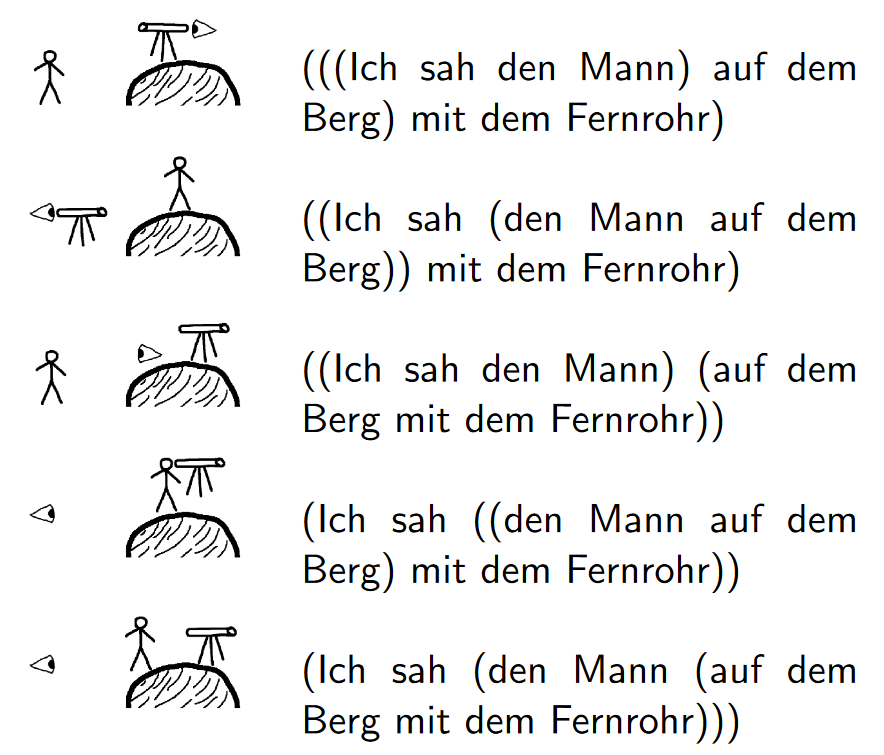
\includegraphics[width=0.65\textwidth]{img/fernrohr.png}  
    \caption[Nichteindeutigkeit nicht-formaler Modelle, KÖNIG Bettina : Vorlesung ''Modellierungsmethoden der Informatik'', \protect\url{http://www.ti.inf.uni-due.de/fileadmin/public/teaching/mod/slides/ws201112/einfuehrung.pdf}, 10.06.2019]{Nichteindeutigkeit nicht-formaler Modelle}\label{fig:fernrohr}
\end{figure} 
Ein \textbf{semiformales Modell} ist teilweise exakt, sprich es verfügt über eine definierte Syntax, spezifiziert aber nicht die ganze Domäne und verfügt über keine semantischen Konstruktionsregeln. Umsetzen lassen sich solche Modelle beispielsweise mit wie etwas ER- oder UML-Modelle,
\\
\textbf{Formale Modelle} verfügen über eine konkrete Syntax und Semantik, die Modelle auf Basis deskriptiver Logiken ermöglicht. Für formale Modelle lassen sich  Algorithmen formulieren, die es erlauben Daten, die durch ein solches Modell beschrieben sind, automatisch zu validieren.
\\
\\
Im Gegensatz zum Computer kann der Mensch auch mit nicht-formalen Modellen arbeiten. Man kann stark strukturierte und formalisierte Modelle, die algorithmisch genutzt werden können, offenen Modellen gegenüberstellen, in die sich ein Mensch hineindenken kann.
\\
Konzeptuelle (konzeptionelle, ist ein Synonym) Modelle (conceptual model) bzw. Informationsmodelle (information model) sind beispielsweise in der Wirtschaftsinformatik von zentraler Bedeutung, da Sie als Schnittstelle zwischen Informatik und Wirtschaftsinformatik besonders gut geeignet sind.\footcite[][S.44-47]{kobler2010qualitat} Ich denke man kann diese genauso auch auf die Digitalen Geisteswissenschaften ummünzen.
\\
\\
huhu\footcite[Vgl][S.99-108]{jannidis2017digital} 
\\
\\
Unterschieden werden eine normative, deskriptive  explorative Funktion eines Modells.
\\
Modellierungen geschieht auf mehreren Ebenen: als modellierte Instanz, das heißt es ist ein Datenabbild eines Gegenstandes oder Textes (Instanz). Datenmodell sind Ausdruck eines Musters, das auf mehrere Instanzen anwendbar ist. Sowie Metamodell, die ein Ausdruck eines Musters ist, das auf mehrere Datenmodelle anwendbar ist, darstellen.
\\
\\
Es gibt vier verschiedene Möglichkeiten, Metamodelle zu gestalten:
\\
\\
Das Entity-Relationship-Modell (ER) baut auf den drei Begriffe Entität, Attribut und Relationauf. Die Entitäten (alle möglichen Untersuchungsobjekte) haben Eigenschaften (“Attribute“) und stehen zu anderen Entitäten in Beziehung („Relation“) Für die Beziehungen spielen die Kardinalitäten/Multiplizitäten eine wichtige Rolle, das heißt, dass ein Objekt unterschiedlich viele Beziehungen haben kann. Die Umsetzung eines ER erfolgt in der Informatik normalierweise in Tabellen, in denen die Beziehungen durch Verweise ausgedrückt werden, und mehrfach vorkommende Daten verringert werden.
\\
\\
Das Graphenmodell baut nur auf zwei Begriffen auf, nämlich der Entity und der Property (Eigenschaft) Rollen; die Eigenschaft ist eine Referenz auf eine andere Entität. Also es geht um „Knoten“ und Verbindungen zwischen Knoten („Kanten“). Entitäten können literal (also eine Zahl oder ein Text) oder eine Ressource (abstrakter Bezeichner für eine Entität) sein. Solche „Graphen“ können sowohl gerichtet als auch ungerichtet sein.
\\
\\
Klassen abstrahieren Entitäten. Das bedeutet, dass jedes Mitglied einer Klasse mindestens eine gemeinsame Eigenschaft mit den anderen Mitgliedern einer Klasse besitzt. Ohne dieser Eigenschaft ist es kein Mitglied. Um das zu bestimmen, muss die Eigenschaft, welche eine Klasse ausmacht, immer genau definiert werden.
\\
\\
Man kann seine Objekte aber auch als Hierarchien modellieren, bei denen Objekte und Eigenschaften Teil eines anderen Objektes sind. Wenn man hier etwas löscht, dann werden auch alle Unterelemente gelöscht.


%%%%%%%%%%%%%%%%%%%%%%%%%%%%%%%%%%%%%%%%%%%%%
%%%%%%%%%%%%%%%%%%%%%%%%%%%%%%%%%%%%%%%%%%%%%
\subsubsection{Forschungsdaten in den Geschichtswissenschaften}

Die Grundlage jeder formalen Verarbeitung sind Daten. Die Definition von Daten lässt sich am besten fassen in der Kontextualisierung mit drei anderen Begriffen: Signal, Information und Wissen. Wo Signale eine physikalische Entität darstellen, beispielsweise eine Lichtwelle, versteht man unter Daten Zeichen zur Verarbeitung und Repräsentation von Information. Noch spezifischer wird der Begriff in der Informatik verwendet. In diesem Fach versteht man unter Daten Informationseinheiten, die für Maschinen lesbar und bearbeitbar sind. Von Information spricht man, wenn Daten in einem bestimmten Kontext interpretiert werden. WERSIG, aus einem kybernetischen Verständnis, spricht bei Information von einer ''\textit{Reduktion von Ungewissheit aufgrund von Kommunikationsprozessen}''\footcite[][S.74]{wersig1971information}. Noch eine Hierarchiestufe höher steht der Wissensbegriff. Wissen, so FAVRE-BULLE, ist gegeben, wenn ein kognitiver Agent, beispielsweise ein Mensch, auf Basis von Information eine Handlung in der Welt setzt.\footcite[][S.93-97]{favre2001information} Folgende Darstellung zeigt die Abhängigkeit dieser 4 Begriffe zueinander, mit einem anwachsen der Komplexität der Struktur, sowie der Anbindung an einen kognitiven Agenten.\footcite[Eine ausführlichere Auseinandersetzung mit den Begriffen Daten, Information und Wissen findet sich in meiner ersten Abschlussarbeit.][Masterarbeit Graz, S.20-28]{pollin2017suchen}
\begin{figure}[H]
\centering
	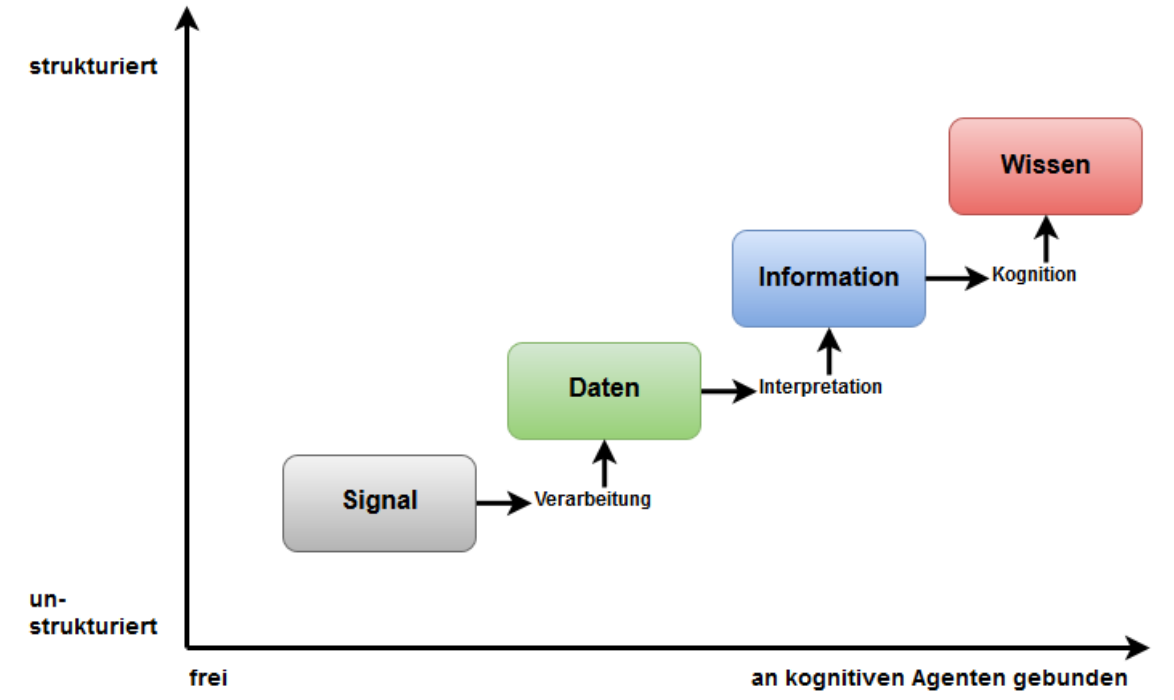
\includegraphics[width=0.85\textwidth]{img/daten.png}  
    \caption[Signal, Daten, Information und Wissen. POLLIN Christopher: Vom Suchen, Stöbern und Finden : Information Retrieval am Beispiel der Digitalen Sammlung des Hans Gross Kriminalmuseums, Masterarbeit Graz, S.21 ]{Signal, Daten, Information und Wissen} \label{fig:daten}
\end{figure} 
Entstehen Daten während eines, oder als Ergebnis eines, Forschungsprozesses so spricht man von \textbf{Forschungsdaten}. Damit werden sowohl Daten aus den Naturwissenschaften (Messdaten aus einem Experiment), Sozialwissenschaften (Interviews) oder den Kulturwissenschaften (dokumentierte Beobachtung) zusammengefasst.\footcite[][09.06.2019]{kindling2013forschungsdatenmanagement}
\\
ANDORFER spricht sich für einen nicht ''\textit{inflationären Gebrauchs dieses Begriffes}'' und einer ''\textit{präzisere   Terminologie}'' im Zusammenhang des Begriffes geisteswissenschaftliche Forschungsdaten aus. Es soll klar definiert sein was man als Forschungsdaten auffasst und was davon ausgeschlossen ist. Weiters soll es bei den für Fachwissenschafter*innen vertraute Begrifflichkeit bleiben und .\footcite[][]{andorfer2015forschungsdaten}
\begin{figure}[H]
\centering
	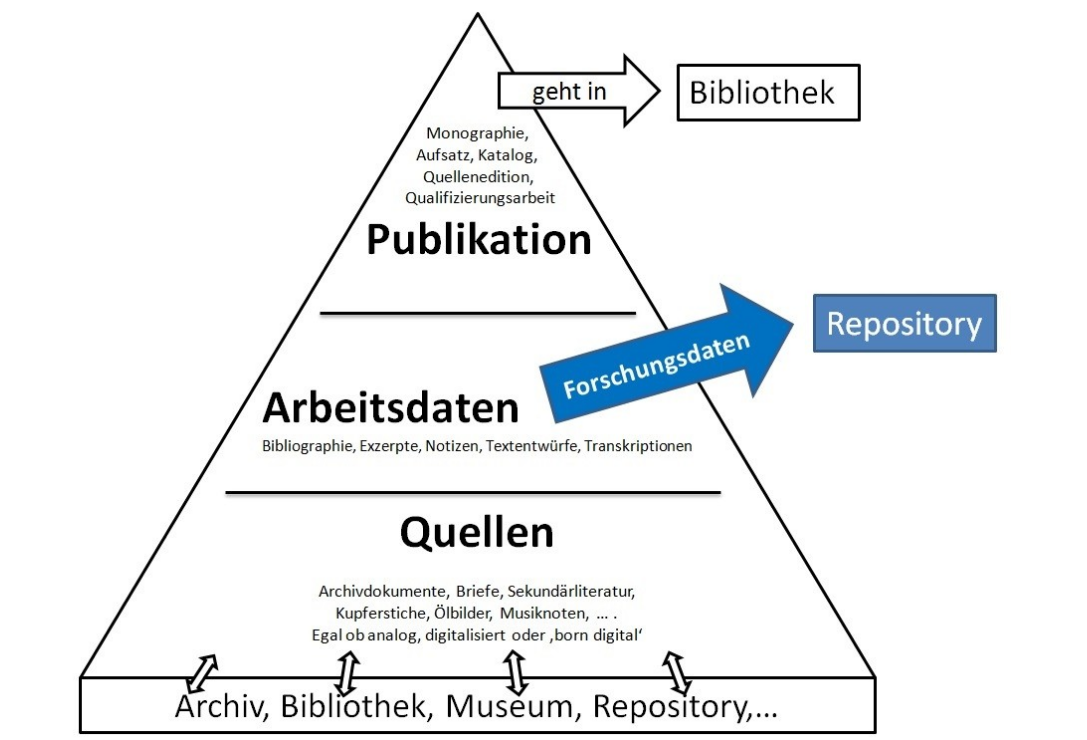
\includegraphics[width=0.85\textwidth]{img/forschungsdaten.png}  
    \caption[Datenpyramide geisteswissenschaftlicher Forschungsdaten im institutionellen Kontext, ANDORFER, Peter: Forschungsdaten in den (digitalen) Geisteswissenschaften: Versuch einer Konkretisierung, 2015, S.14]{Datenpyramide geisteswissenschaftlicher Forschungsdaten im institutionellen Kontext nach ANDORFER} \label{fig:forschungsdaten}
\end{figure} 
Für die Geisteswissenschaften und im speziellen für die Geschichtswissenschaften, in denen viel stärker hermeneutischer Prozess  im Vordergrund stehen, ist der Begriff nicht eindeutig. HILTMANN sieht einen engeren und einen weiteren  Begriff von Forschungsdaten in den Geschichtswissenschaften. Im engeren Sinne versteht man Metadaten zu und Annotationen von historischen Quellen in all ihren Ausprägungen. Als Beispiel ist die archivalische Erschließung eines Quellenkorpus angeführt, damit die Verwahrung und Auffindbarkeit für eine potentielle wissenschaftliche Auseinandersetzungen ermöglicht wird. Im weiteren Verständnis kann alles, das digital vorhanden ist zur historischen Quelle und somit zu relevanten Daten für dei Geschichtswissenschaft werden.\footcite[Vgl.][09.06.2019.]{hiltman2018forschungsdaten}
\\
Im Zuge dieser Arbeit soll aber dem engeren Begriff folge geleistet werden. Forschungsdaten wie Geschichtswissenschaften sind sowohl innere wie äußere merkmale historische Quellen wieso adverben speichert werden verfügung stehen die interpretierbar und Maschinen verarbeitbar. 

%%%%%%%%%%%%%%%%%%%%%%%%%%%%%%%%%%%%%%%%%%%%%
%%%%%%%%%%%%%%%%%%%%%%%%%%%%%%%%%%%%%%%%%%%%%
\subsubsection{Modelle in den Geschichtswissenschaften}

Damit Forschungsdaten nachnutzbar und nachvollziehbar sind bedarf es eines mitgelieferten Modells. Diese Modelle wiederum müssen auf Standards beruhen. Es ist zeitensiv die Datenmodelle andere zu verstehen und oft ist es leichter sein eigenes Modell zu entwickeln. Ein generelles Problem mit Informationssystem und Forschungsdaten ist, dass sie nur für eine bestimmte Fragestellung bzw. ein bestimmtes Projekt entwickelt wurden. Werden bei der Generation der Forschungsdaten aber bereits Konzepte und Standardisierungen verfolgt, so fällt es leichter die ''Datensilos'' zu verlassen und die Nachnutzung zu fördern. 
\\
Eine erste Form der Standardisierung in den (digitalen) Geisteswissenschaften ist die Text encoding Initiative (TEI). Wenn auch Umsetzungen der TEI nicht einem 'klassischen' Standard entsprechen, so sind sie Überlegunen, wie man Text strukturieren und annotieren kann, sehr wohl standardisiert. 
\\
Es ist eine Notwendigkeit, dass Standards auf der einen Seite ausdrucksstark sein müssen, um die unterschiedlichen Problemstellungen fassen zu können, anderenseits es sich aber daraus formale Modelle ableiten lassen müssen. THALLER fordert deswegen, dass die Standards zur Beschreibung von Modellen eher beschreibend statt  vorschreibend sind.\footcite[][S.204]{thaller2017need}

%%%%%%%%%%%%%%%%%%%%%%%%%%%%%%%%%%%%%%%%%%%%%

\section{Historische Rechnungsbücher als Quelle}
\label{Rechnung}

In diesem Kapitel wird das Rechnungsbuch als historische Quelle dargestellt und sowohl inhaltliche wie auch äußerliche Eigenschaften festgemacht. In einem weiter Schritt wird dann auf konkrete digitalen Editionsprojekte von Rechnungsbüchern eingegangen.
\\
Bei Rechnungsbüchern handelt es sich um pragmatisches, aus dem Alltag der Menschen stammendes Schriftgut, das zur Dokumentation und als Gedächtnisstütze diente, bis eine Schuld getilgt wurde. Zu meist auf Papier und ohne übergeordneten Standards verfasst, folgte sie keinen repräsentativen Zweck. Dennoch haben sie zumeist eine einheitliche Struktur, die zeigt, das es sich um ein ''\textit{Werkzeug des Alltages}'' gehandelt hat, damit es auch für andere verständlich und nachnutzbar ist. GLEBA und PETERSEN heben eine Vielfalt der Inhalte in Rechnugnsbüchern, sowie die Möglichkeiten der ''\textit{interdisziplinären Erschießung der Quelle 'Rechnungsbuch'}'' hervor. Die Herausforderungen der Erschließung der Quelle sind vielfältig: Maß-, Größen- und Gewichtsordnungen und Information zu Geldwerten sind sehr stark an Region und Zeit gebunden. Dennoch lassen sich viele Forschungsfragen aus solchen Quellen ableiten: wie haben sich Güter, Dienstleistungen und Geldbeträge über die Zeit hinweg verändert, welche wirtschaftlichen Abhängigkeiten zwischen Akteuren gibt es? Rechnungsbücher gehen ''\textit{weit über wirtschafts- und verwaltungsgeschichtliche
Aspekte hinausgehen}''\footcite[Nach KLAPP,][S.14]{bauch2015daten} und so haben Fragestellungen dieser Art weitere soziale, gesellschaftliche und wirtschaftliche Implikationen, die uns ein Verständnis geben können, wie das Leben der Menschen in der Vergangenheit ausgesehen haben kann.\footcite[][S.7-10]{gleba2015einleitung}
\\
\\
BRUCH sieht Rechnungsbücher sehr geeignet dafür Daten zu liefern, damit sie mit quantitativen Methoden weiterverarbeitet werden können.\footcite{bauch2015daten}
\\
\\
MEDEA-Paper:
Historical accounting documents have taken many forms over the course of human history, and
their formats have changed in ways that have not always been reflected in the historical
literature. While a shorthand reference to the development of so-called double entry accounts
based on the practices of early modern Italian merchants might prevail among historians of the
modern era, considerable evidence demonstrates a more nuanced process of change over time. In
fact, historians have used the term “accounts” for a wide range of primary sources. Long before
the fifteenth century, people all over the world tracked exchanges of goods, services, and rights
by writing on a variety of materials that included clay and wax tablets, slate, tallies, papyrus,
parchment, and paper, and they used a range of tools that were appropriate to these different
materials. At various times and places, the people making these records had literacy skills
ranging from basic numeracy through full literacy; their purposes in creating the records
extended from simple memory aids through complex professional evaluations. The common
element among these highly differentiated sources was their focus on economic activities. Thus,
we can deduce that the form and inner structure of the accounts evolved in relation to available
materials and tools, in association with diverse purposes, and in connection to the development
of economic activities.
Historians have demonstrated that those responsible for keeping track of the funds of cities,
estates, businesses, charities, and other human organizations developed their accounting
practices as they encountered new situations and problems. Medieval and early modern accounts
from French- and German-speaking regions reveal some of the processes of this non-linear,
locally influenced development (Arlinghaus 2000, Mersiovsky 2000). And research on
nineteenth-century business accounts has shown that only in the final decades of the century did
accounting become a professional pursuit in which such contemporary notions as cost accounting
and depreciation of business machinery were standard management principles that reputable
firms and organizations were expected to follow (McGaw 1985, Yates 2000). In the following
four examples, MEDEA participants illustrate areas where digital scholarly editions of accounts
can add to knowledge about the evolution of accounting practices as well as about daily life and
the sorts of factors that have been the subject of social and economic history for the past eighty
years.\footcite[][S.2]{tomasekmedea}
\\
\\
Historische Rechnungsbüchern sind einen Teil einer Menge von Primärquellen, die Aufzeichnungen von Handel mit Waren und Dienstleistungen darstellen. Sie werden seit längerer Zeit als Primärdatensätze für historische Forschung genutzt. Sie liefern reichhaltige und strukturierte Daten, die oft längere Zeiträume abdecken und die als Aggregation vieler Einzelinformationen enthalten zu Beantwortung unterschiedlicher Forschungsfragen herangezogen werden können. Sie beinhalten beispielsweise Information über den Kauf und Verkauf von Waren, Werkzeugen und Rohstoffen eines bestimmten Gewerbes, sowie über die ausgezahlten Löhne von Arbeitnehmern*innen. Eine andere Art von Rechnungsbüchern stellen Haushaltskonten dar. Diese beziehen sich auf den Kauf von Lebensmittel und Bekleidung sowie für Zahlungen für Dienstleistungen in Form von Kochen, Waschen oder andere Haushaltsarbeiten.   HFRs im Zusammenhang mit der Haushaltsführung auch im Zusammenhang mit der Haushaltsführung enthalten Listen der für Hausarbeit gezahlten Löhne, und solche Listen finden sich manchmal auf der Seite Rückseiten von Taschenkalendern und nicht in formalen Kontenbüchern oder Ledgern. In Regionen wo Arbeiter versklavt wurden, finden sich HFRs in den Buchhaltungsbüchern und in der persönlichen Aufzeichnungen über Sklavenhalter und Sklavenhändler.\footcite[][S.2]{tomasek2013encoding}
\\
Eine Transkription allein reicht nicht aus um die unterschiedlichen Dimensionen einer solchen Quelle abzudecken: die linguistische/textuelle, die quantifizierbare und die semantische Dimension. Für Forschungszwecke unterliegen historische Quellen einem Transformationsprozess hin zu (vernetzten) Informationsquellen, die in verschiedenen Forschungsszenarien genutzt werden können. Um dies zu veranschaulichen, werden drei Fallstudien von Projektpartnern und ihren jeweiligen Forschungsinteressen diskutiert, die weit über wirtschaftliche und administrative Aspekte hinausgehen.
\\
\\
Händler haben finanzielle Aufzeichnungen geführt, um Käufe und Verkäufe von Waren seit den Handelsökonomien des alten Mesopotamiens zu verfolgen, und der Impuls, regelmäßige Konten zu führen, führte zu Standards für die Erfassung von Finanzinformationen. Im Laufe der Jahrhunderte boten verschiedene einflussreiche Texte gewöhnlichen Geschäftsleuten die Möglichkeit, zu lernen, wie man das macht. Für das frühneuzeitliche Europa skizzierte Fra Luca Pacioli in seiner Abhandlung The Rules of Double-Entry Bookkeeping von 1494 Rechnungslegungsgrundsätze, die die Handelsrechnung in ganz Europa beeinflussten. Mitte des achtzehnten Jahrhunderts veröffentlichte der schottische Mathematiker John Mair ein einflussreiches Lehrbuch mit dem Titel 
Buchhaltungsmethodik; oder, eine methodische Abhandlung von Handelskompten, nach der italienischen Form. Bei der Präsentation von Pacioli's System für Englischsprachige durchlief Mair's Text zahlreiche Ausgaben zwischen den folgenden Sprachen 1736 und 1808. \footcite[][S.3]{tomasek2013encoding}


%%%%%%%%%%%%%%%%%%%%%%%%%%%%%%%%%%%%%%%%%%%%%
%%%%%%%%%%%%%%%%%%%%%%%%%%%%%%%%%%%%%%%%%%%%%
\subsection{Finanztransaktionen}

\textit{Extensible Business Reporting Language }(XBRL)\footcite{engel2003extensible} ist ein XML-basierter Standard und frei verfügbare Sprache für die Beschreibung und den Austausch inhaltlicher und technischer Information der Geschäftsberichterstattung. XBRL verwendet verschiedenen Spezifikationen und das Herzstück bildet ein \textit{instance document}, das die finanziellen Fakten beschreibt und eine \textit{taxonomy} das die Konzepte erfasst. Kodierung eines Finanzbericht in XBRL erfordert die Verbindung von Instanzdokumenten mit Taxonomien und zugehörige \textit{Linkbases}, die Sammlungen von eingehenden und externen Links enthalten. CLIFFORD et. al führen an, dass es für die Beschreibung von Transaktionen in historischen Rechnungsbüchern geeignet ist, kritisieren aber das es für die Foramlisierung historischer Daten nicht entwickelt wurde. Beispielsweise ist es nicht möglich historische Währungen in XBRL zu beschreiben, da nur die durch ISO 2015 definierten Währungen erlaubt sind.\footcite[][S.7-9]{tomasekmedea}.

%%%%%%%%%%%%%%%%%%%%%%%%%%%%%%%%%%%%%%%%%%%%%
%%%%%%%%%%%%%%%%%%%%%%%%%%%%%%%%%%%%%%%%%%%%%
\subsection{DEPCHA}
\label{DEPCHA}

Daten - aus unterschiedlichen Formaten - sollen auf einer gemeinsamen Plattform zusammengeführt werden und adäquate Formen des Retrievals, Discoverys und der Visualisierung eröffnen, um die Arbeit mit den Quellen zu erleichtern. Die Überführung nach RDF auf Basis der im Projektkontext entwickelten \textit{Bookkeeping-Ontologie}, die Transferprozesse historischer Rechnungsbücher formalisiert, erlaubt die Interoperabilität, Verlinkung und Zusammenführung der Informationen im Sinne des \textit{Web of Data} und \textit{Linked Open Data}.


\subsubsection{The George Washington Financial Papers}
The George Washington Financial Papers (1748-1799) 3 gives insight into the life of
George Washington and other topics such as the material culture, social history,
manufacturing and agriculture. The financial papers exist as digital edition, created and
published via an open-source, Drupal 4 based editorial platform, and aim to make
Washington’s records freely accessible. The platform allows editing and publishing
financial documents and gives the users the possibility to perform simple analytical
functionalities. Samples of research questions that could be of interest to historians are:
How much money did Washington spent annually and for which specific commodities?
Which role slave trade plays in his business? How did the price of certain commodities
fluctuate? What did the network of partners look like and who did business with him?
How was the value of tobacco calculated through different currencies [St14]?

\subsubsection{Stageville}

\subsubsection{The Wheaton Accounts}

Die \textit{Wheaton Family Papers} umfassen mehrere Bücher im Zeitraum von 1828 bis 1859, die unter anderem die finanziellen Geschäfte von \textit{Laban Morey Wheaton} und seiner Familie, einem Geschäftsbesitzer eines \textit{dry goods store} aus Norton, Massachusetts in den Vereinigten Staaten von Amerika, dokumentieren. Unter \textit{dry goods} versteht man einen aus dem 17. Jahrhundert stammenden historischen Begriff, der je nach Region leicht unterschiedliche Güter zusammenfasst. Darunter werden im Allgemeinen aber Produkte verstanden, die ''trocken'' sind, wie etwa Textilien, Konfektionskleidung, Tabak oder bestimmten Lebensmittel, wie etwa Kartoffel.\footcite[Definition von \textit{Dry Goods}, \protect\url{https://chestofbooks.com/reference/Dictionary-of-Dry-Goods/Dry-Goods.html}, 23.05.2019, Vgl.][]{cole2015complete}
\\
Die Stadt Norton ist eine charakteristische landwirtschaftlich und von Manufakturen geprägte Kleinstadt im Nordosten der USA im Hinterland der regional bedeutenden Häfen Boston, New Bedford, Newport, and Providence. In einer Geschichte der Stadt Norton von CLARK wird \textit{Laban Morey Wheaton} namentlich genannt. Er lebte von 14.September 1796 bis 1865, hat Rechtswissenschaften an der \textit{Brown University} studiert und jahrelang als \textit{Postmaster of Norton} gearbeitet. Er war politisch aktiv und war Vertreter im \textit{Massachusetts General Court}, sowie Mitglied im \textit{Massachusetts Governor's Council}. Er war verheiratet und Angehöriger des Kongregationalismus, einer Form der christlichen Gemeindeverfassung. Die Wheaton Familie besaß eine Milchviehherde sowie Fabriken zur Produktion von Baumwollwatte, die \textit{Wheaton Manufacturing Company,} und eine zur Produktion von Strohhüten\footcite[][S.6]{tomasek2013encoding} und so gehörte Laban Wheaton zu einem der wohlhabendes Männer der Stadt. Sogar ein Portrait von ihm ist bei CLARK überliefert.\footcite[][S.496]{clark1859history} 
\begin{figure}[H]
\centering
	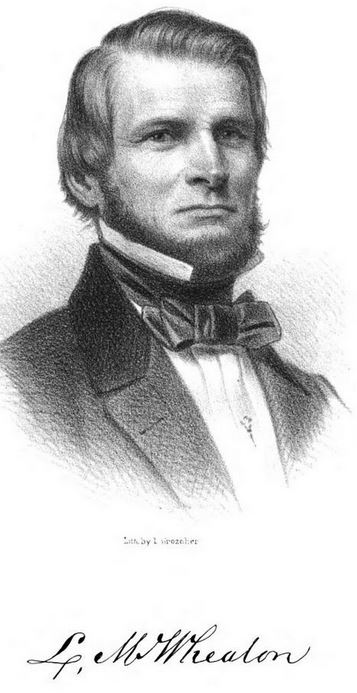
\includegraphics[width=0.2\textwidth]{img/LMwheaton.jpg}  
    \caption[Portrait von Laban Morey Wheaton, Vgl. CLARK, George Faber: A History of the Town of Norton, Bristol County, Massachusetts, from 1669-1859.
Crosby, Nichols, and Company, and author at Norton, 1859, S.497.]{Portrait von Laban Morey Wheaton} \label{fig:LMwheaton}
\end{figure} 
Aus diesem Kontext heraus, der über \textit{Laban Morey Wheaton} überliefert ist kann man die These aufstellen, dass er ein mächtiger Mann war. Auf der einen Seite politisch aktiv und politischer Vertreter, auf der anderen Seite vermögend und Besitzer mehrere Immobilien und eines Geschäftes. Gerade der im \textit{daybook} dokumentierte Verkauf von Gütern, in dem Menschen Lebensmittel im Austausch für Arbeit erwerben, zeigt eine gewisse Machtposition. Denn die, nicht vollständig überlieferten, Rechnungsbücher von Wheaton zeigen nicht nur Angaben zu Gütern, Dienstleistungen und Geldbeträgen in den einzelnen Transaktionen, sondern auch Namen einer Vielzahl von Individuen und ihrer Familien, die in Beschäftigungsverhältnissen mit Wheaton stehen, Objekte und Gebäude mieteten oder Handel betrieben. TOMASEK führt an, dass diese Rechnungsbücher detaillierte Informationen über das tägliche Leben der Einwohner*innen einer Stadt in New England, geprägt durch eine gemischte Land-, sowie Industriewirtschaft im zweiten Quartal des 19. Jahrhunderts, darstellen.\footcite[][S.5]{tomasekmedea}
\\
\\
Das \textit{Wheaton College Massachusetts} stellt die \textit{Wheaton Family Papers} Dokumente in ihrem digitalen Repositorium online zur Verfügung.\footnote{Wheaton Family Papers, \url{https://digitalrepository.wheatoncollege.edu/handle/11040/7928}, 19.05.2019.} 
\\
Die wissenschaftliche Auseinandersetzung erfolgt durch Kathryn Tomasek, Professorin für Geschichte am \textit{Wheaton College Massachusetts}. Im Zuge des Projektes \textit{The Wheaton College Digital History Project} wurden Teile der Wheaton Paper, darunter beispielsweise das oben angeführte \textit{daybook} gemeinsam mit Studierenden transkribiert und mit dem Standard der Text Encoding Iniative (TEI) ausgezeichnet und im Sinne einer Vorarbeit einer digitalen Edition ediert. Der Fokus dieser Arbeiten liegt auf der Erschließung der einzelnen Transaktionen und der damit verbundenen Personen, Güter und Dienstleistungen.\footcite[Vgl. TOMASEK Kathryn: The Wheaton College Digital History Project: Undergraduate Research in a Local Collection, \protect\url{https://writinghistory.trincoll.edu/teach/wheaton-college-digital-history-project-tomasek/}, 23.05.2019.][S.379]{alexander2012should} Teile davon wurden im Zuge des DEPCHA Projektes für die Umsetzung eines Prototyps zur Publikation von semantisch angereicherten, digitalen Edition von Rechnungsbüchern verwendet.
\\
\\
Verkauf und Kauf von Gütern des täglichen Lebens listet und ein \textit{Ledger}, ein Hauptbuch, das die Finanzflüsse an einer zentralen Stelle zusammenfasst transkribiert und mit der TEI ausgezeichnet.\footcite[][]{tomasek2013encoding}
\\
\\
Im Alltag einer Kleinstadt wie Norton zu dieser Zeit trafen sich Menschen regelmäßig und man kannte sich persönlich. Die systematische Buchführung bot Laban Morey Wheaton eine Möglichkeit seine Geschäfte von seinen persönlichen Interaktionen zu trennen. Zur Dokumentation dieser Geschäfte führte er mehre Bücher nach dem Prinzip der Doppelteebuchführung und trennte HABEN und SOLL auf zwei Bücher. Transaktionen zwischen lokalen Geschäftspartner*innen und seinen Kund*innen wurden chronologisch im \textit{Daybooks} erfasst, jeweils mit einem Verweis in der linken Spalte auf die Seite im Hauptbuch, auf der der Geschäftsmann die laufende Schuld des Kunden und die Zeiten, zu denen die Schuld beglichen wurde, erfasst hat.\footcite[][S.7-9]{tomasek2013encoding} Folgende Abbildung \ref{fig:wheaton} zeigt Seite 100 und 101 des \textit{Daybooks}. An diesem Beispiel soll nun die grundlegende Struktur dieser Quelle beschrieben werden. Die linke Seite beginnt mit einer Überschrift ''\textit{Norton Tuesday Sept 6 1831}''. Die ersten Einträge in dieser tabellarischen Struktur beziehen sich nun auf den 6. September des Jahres 1831. An diesem Tag hat "\textit{Wheaton Wheeler}" einen halben ''\textit{Burell Corn}'', also ein halbes Büschel Mais, für den Geldbetrag von 50 Cent erworben. Die Zahl ''393' an der der ersten Spalte  referenziert auf das Hauptbuch und verweist auf eine Seite wo Information zum Satus der Transaktion vorzufinden sind und zeigt somit die Doppeltebuchführung. Hier lassen sich auch Wörter wie '\textit{Bill}'', ''\textit{Paid}'' oder ''\textit{Settled}'' vorfinden, die zeigen, dass der Status einer Transaktion'auf Rechnung erfolgte, bereits bezahlt oder anderweitig beglichen wurde. Die mittlere Spalte nennt die zweite Person, neben Laban Wheaton, die an der Transaktion beteiligt ist: den Käufer. Jeder hier angeführte Oerson steht als in einem Geschäftsverhältnis mit Wheaton. jeweils darnter werden die einzelnen Transaktionen gelistet In den 4 Spalten rechts, werden die Geldbeträge gelistet: in der ersten Spalte die Dollar und in der zweiten die Cent. Sowie bei der Zusammenfassung mehrere Transaktionen zu einer Person auch eine Summe.
\\
Im Textfluss lassen sich zwischen den Einträgen entweder einfache Zahlen ''12'', ''24'' oder neue Tagesdaten finden, die eben nun alle folgende Transaktionen einem neuem Datum zuordnen. So steht ''12'', ''24'' auf diese 100 f+r den 12. und 24.September und ''Oct 8th 1831'' ordnet alle folgenden Einträge  dem 8. Oktober 1831 zu.
\\
Rechts neben den Akteuren in den Einträgen lässt sich meistens ein ''D'' bzw. ''Dr'', seltener ein ''C'' bzw. ''Cr'' vorfinden, für ''Debitor'' und ''Creditor'' steht. Dies markiert eine Transaktion mit diesem Partner, das sie auf die HABEN bzw. die SOLL Seite gebucht wird.
\begin{figure}
\centering
	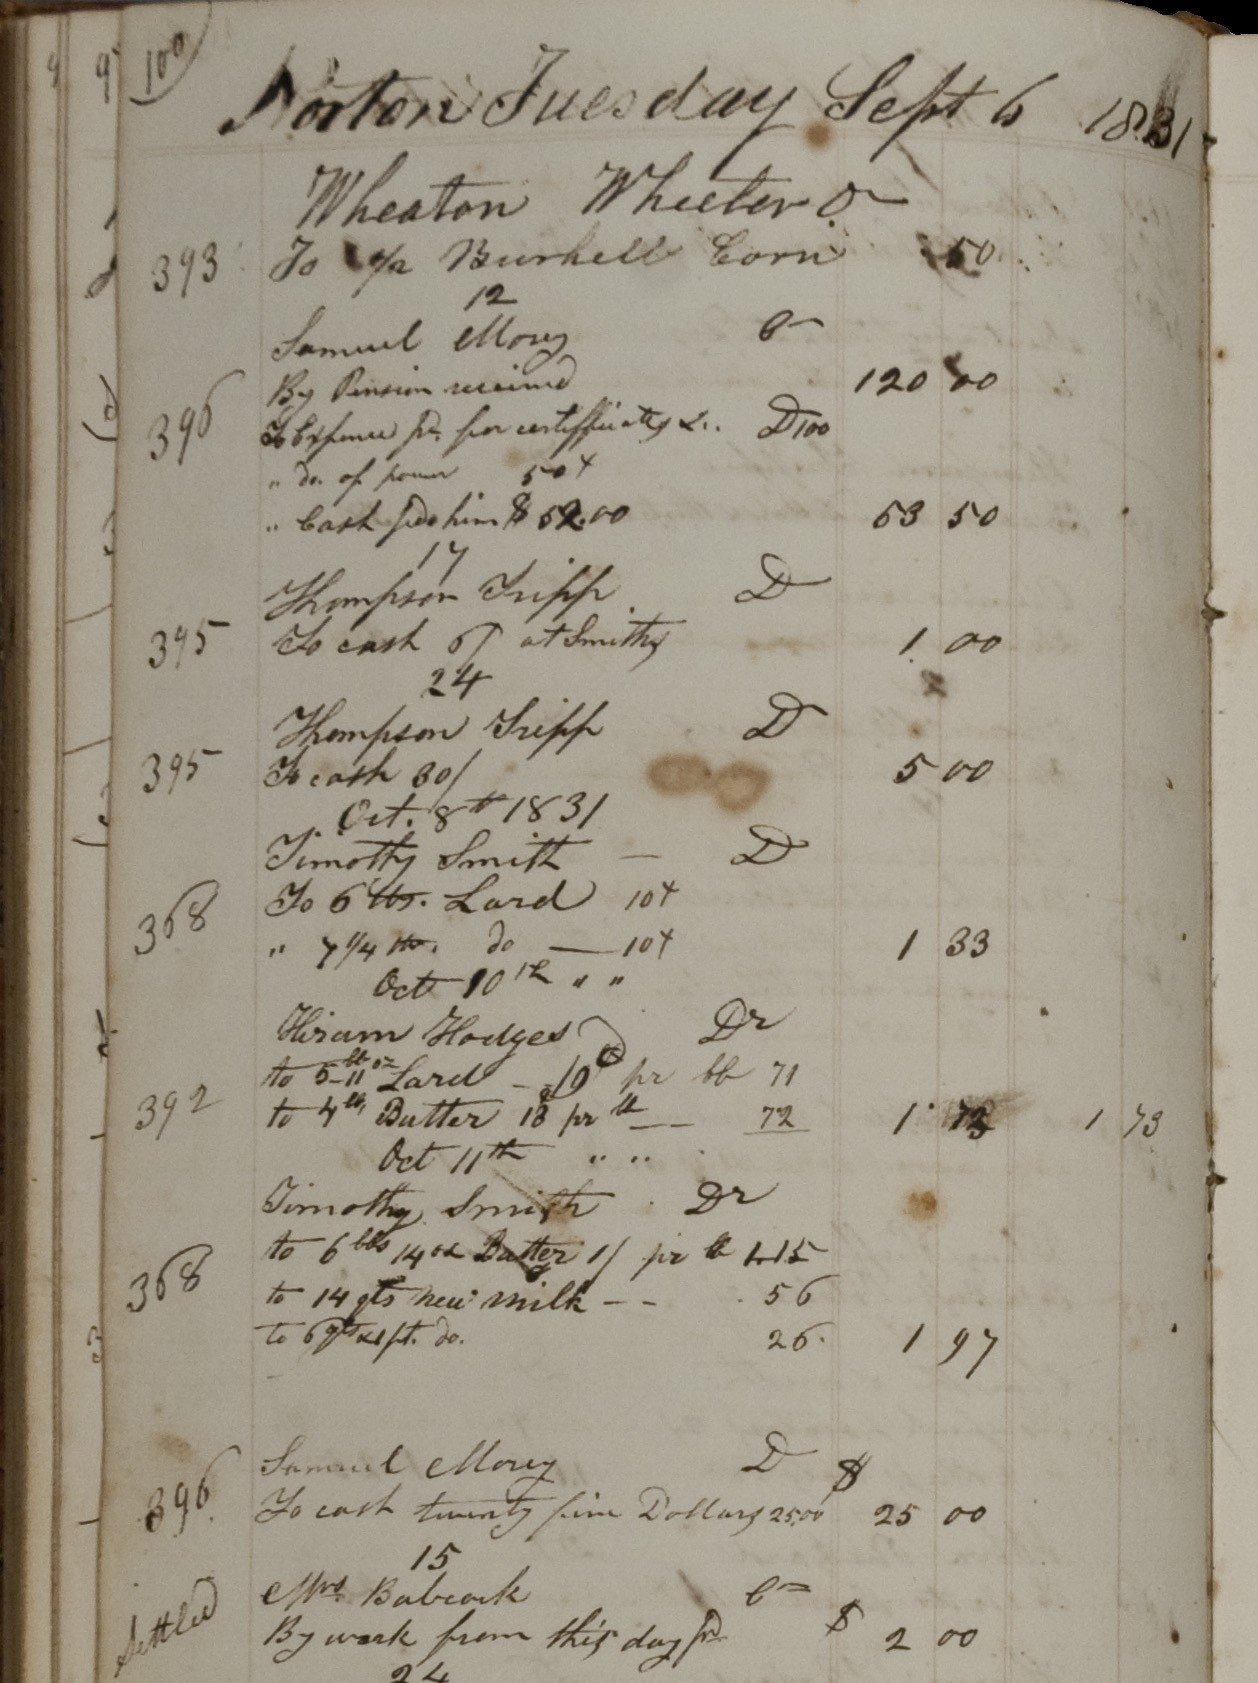
\includegraphics[width=1\textwidth]{img/wheaton_100_101.jpg}  
    \caption[Seite 100 des \textit{Daybook, \protect\url{http://hdl.handle.net/11040/17982}}, 1828-1859]{Seite 100 des \textit{Daybook}, 1828-1859a} \label{fig:wheaton}
\end{figure}
\\
Die vollständige Transkription der ersten 8 Einträge der Seite 100. Diese zeigen die soeben beschriebenen Strukturen.
\\
\\
\begin{tabular}{clcc}
 \textbf{Norton Tuesday Sept 6 1831}\\
    & Wheaton Wheeler & &\\
393 & Dr To 1/2 Burhell Corn & & 50 \\
    & 12 & &\\
    & Samuel Morey  Cr  & &\\
396 & By pension received & 120 & \\
    & To Expense pd. for certificates L. D100 & &\\
    & "Do. of power 50x & &\\
    & " Cash pd. him \$62.00 & 53 & 50\\
    & Thompson Tripp  DR  & &\\
395 & To cash 6/ at Smiths & 1 & 00\\	
    & 24 & &\\
    & Thompson Tripp  DR & &\\	
395 & To cash 30/ & 5  & 00\\		
Oct. 8th 1831\\
    & Timothy Smith DR & &\\
368 & To 6 lb. Lard 10x 6 lb. Lard"7 1/4 lb do 10x & 1 & 33 \\
Oct 10th " "\\
    & Hiram Hodges Dr & &\\
392 & To 5 lb11 oz Lard - 19d pr lb\\
    & 71 5 lb11 oz Lard To 4 lb Butter 13 pr lb 72 & 1 & 73\\
Oct. 11th " "\\
    & Timothy Smith  Dr& &\\
368 & To 6 lbs 14 oz Butter 1/ pr lb 1.15 & & \\ & To 14 Qts New Milk 56 & &\\
& To 6 Qts \& 1 Pt. do 26 & 1 & 97 	\\	
    & Samuel Morey DR & &\\
396 & To cash twenty five dollares 25.00 & 25 & 00\\
    & 15 & & \\	
    & Mrs. Babcock DR  & & \\		
Settled & By work from this day pd & \$2 & 00
\end{tabular}
\\
\\
TOMASEK verfolgt dabei einen TEI/XML-Ansatz, um drei Ebenen dieser Quelle zu beschreiben. Das Layout, die textuelle Struktur der Quelle und die abstrakte Ebene, inhaltliche Ebene der Transaktionen. Letztere ist nur schwer durch die TEI Markup beschreibbar.
\\
Es erweitert den Bereich der Fragen zu historischen Narrativen und geografischen Informationen. Es ist interessant zu folgen.
eine Person oder eine Familie, wie sie im Laufe der Zeit im Tagesbuch erscheinen und ihre Lebensweise rekonstruieren. 
sozialer Hintergrund für eine historische Erzählung. Gleiches gilt für geografische Informationen.
die Möglichkeit, geografische Beziehungen von Personen oder die Herkunft von Waren zu verfolgen.
\\
\\
Ziel der Masterarbeit soll es nicht sein die Projektinhalte zu dokumentieren, sondern sich mit theoretischen und praktischen Fragestellungen zu formaler Modellen und formaler Methoden in den Geschichtswissenschaften  auseinanderzusetzen, wiewohl Quellen, Workflows und Daten aus dem DEPCHA Projekt einfließen sollen.


%%%%%%%%%%%%%%%%%%%%%%%%%%%%%%%%%%%%%%%%%%%%%
\section{Web of Data}
\label{WebofData}
Das Web of Data kann als Stack an Standards und Technologien aufgefasst werden. Flexibel und ausdrucksstark auf der einen Seite und mit dem Ziel maschineneverständliche Information anzubieten, scheint es geeignet als Standard um Modelle zu beschreiben und zu verteilen.

%%%%%%%%%%%%%%%%%%%%%%%%%%%%%%%%%%%%%%%%%%%%%
%%%%%%%%%%%%%%%%%%%%%%%%%%%%%%%%%%%%%%%%%%%%%
\subsection{Geschichte und Vision des Web of Data}

Beim \textit{TED Talk} im Jahre 2009 fordert Tim Burners-Lee das Auditorium auf mit ihm gemeinsam die Worte zu rufen: ''\textit{Raw Data Now!}''.\footnote{BERNERS-LEE Tim: The Next Web, \url{https://www.ted.com/talks/tim_berners_lee_on_the_next_web?language=de}, 05.04.2019.} Die Vision von Burners-Lee, dem Erfinder des World Wide Web, ist das sogenannte \textit{Semantic Web}:
\\
\\
''\textit{The Semantic Web will bring structure to the meaningful content of Web pages, creating an environment where software agents roaming from page to page can readily carry out sophisticated tasks for users.}''\footcite[][S.3]{berners2001semantic}
\\
\\
Im Gegensatz zum klassischen Web, das als ein Web von Dokumenten betrachtet werden kann, versucht das \textit{Web of Data} Daten aus unterschiedlichen Quellen zu integrieren und miteinander zu verknüpft. Daten sollen so vorliegen, dass nicht nur Menschen diese in neuen Kontexten nutzen können, sondern auch Softwareagenten. Maschinen sollen in der Lage sein selbständig die Struktur von Daten ''verstehen'' zu können, um bestimmte Aufgaben umsetzen zu können. Oder anders formuliert sollen Maschinen Inhalte im Web soweit verarbeiten können, dass Automatisierung auf Ebene der Bedeutung möglich ist. Ein konkretes Anwendungsszenario, das mit Hilfe des \textit{Web of Data} umgesetzt werden könnte, wären verbesserte Suchfunktionalitäten für Informationssysteme, die auch die semantische Ebene miteinbeziehen. TOCHTERMANN und MAURER führen ein Beispiel eines Informationsbedürfnisses einer Person an, die gerne einen Termin mit einem Arzt in Graz vereinbaren möchte, der gleichzeitig auch ein Homöopath ist. Diese Person stellt eine Suchanfrage in einer dafür geeigneten Suchmaschine, bestehend aus 4 Wörtern: ''Ärzte, Homöopathie, Stadt Graz''. Da in einer klassischen Suchmaschine nur das Vorkommen der Wörter berücksichtigt wird, muss die suchende Person sich noch durch die angezeigten Suchergebnisse arbeiten, bis sie den passendebn Treffer gefunden hat. Eine Suchmaschine im \textit{Web of Data} ist in der Lage sogenannte Wissensbasen zu befragen, um welche Begriffe es sich hinter den Zeichenketten handelt.\footcite[S.1-2]{pellegrini2006semantic} 
\\
 Dabei handelt es sich aber weder um Maschinen die selbstständig lernen, oder gar eine künstliche Intelligenz, sondern um formalisiertes, maschinenlesbares Wissen. Der Wissensbegriff in diesem Zusammenhang entspringt einer informationswissenschaftlichen Perspektive wie bei WERSIG, KUHLEN oder FAUVR-BULLE.

a
\footcite[S.1-6]{pellegrini2006semantic}


%%%%%%%%%%%%%%%%%%%%%%%%%%%%%%%%%%%%%%%%%%%%%
%%%%%%%%%%%%%%%%%%%%%%%%%%%%%%%%%%%%%%%%%%%%%
\subsection{Web of Data Stack}

Um diese - noch nicht erreichte Vision - in die Tat umzusetzen bedarf es mehrere aufeinander aufbauender technischer Grundlagen, die sich im \textit{Semantic Web Stack} manifestieren. Auf dessen Basis, dargestellt in Abbildung \ref{web_stack}, soll in diesem Kapitel die grundlegenden Technologien und Standards des \textit{Web of Data} erörtert werden.
\begin{figure}[h]
  \centering
	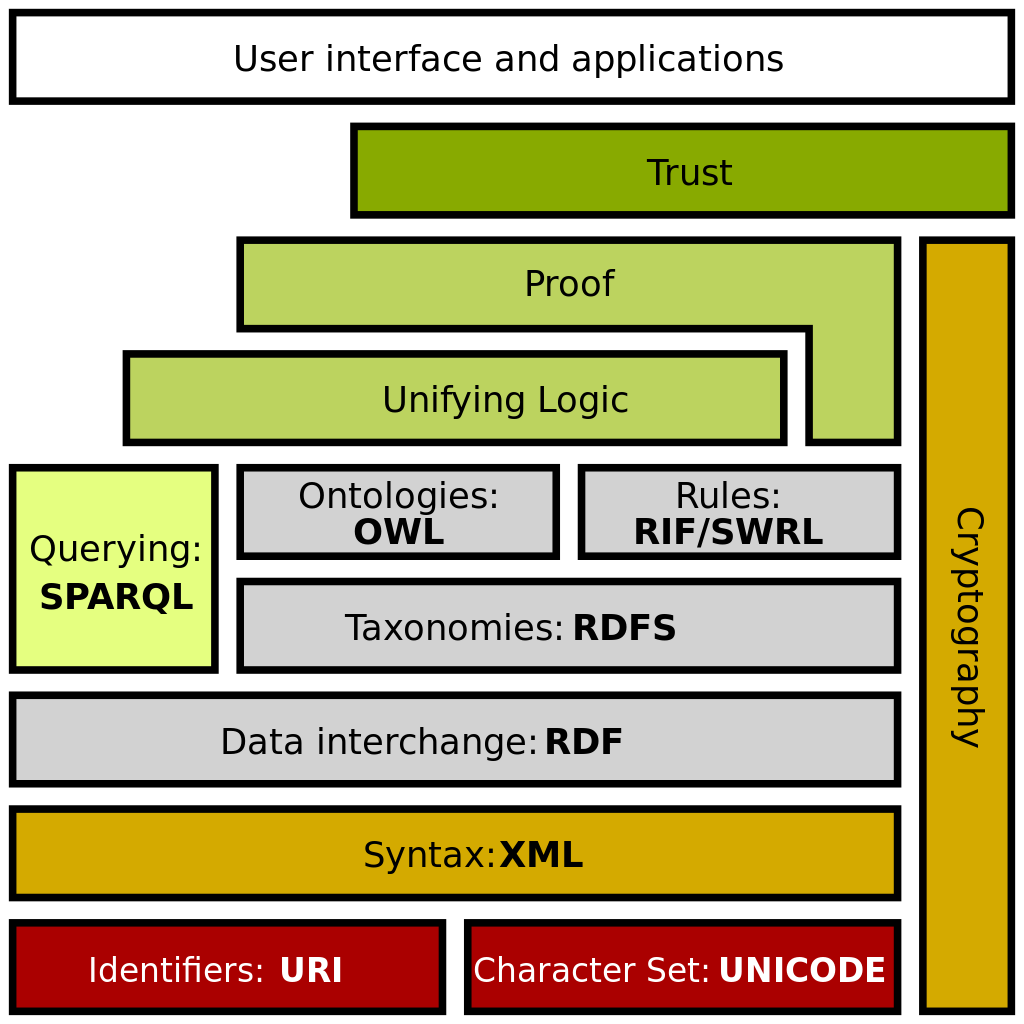
\includegraphics[width=0.65\textwidth]{img/web_stack.png}  
    \caption[Visualisierung eines Graphen auf Basis eines RDF-Datensatz, \protect\url{https://www.w3.org/TR/rdf11-primer/}, 10.04.2019.]{Visualisierung eines Graphen auf Basis eines RDF-Datensatz.}
  	\label{fig:web_stack}
\end{figure}

Das Semantic Web ist nicht erreicht. Zumindest nicht für die Allgemeinheit. Die großen Internetriesen hingegen verfügen über ''ihre Semantic Web'', in denen sie ihre eigenen Agenten mit ihrer großen Datenmenge arbeiten lassen.\footnote{\url{https://twobithistory.org/2018/05/27/semantic-web.html}}




%%%%%%%%%%%%%%%%%%%%%%%%%%%%%%%%%%%%%%%%%%%%%
%%%%%%%%%%%%%%%%%%%%%%%%%%%%%%%%%%%%%%%%%%%%%
\subsubsection{Resource Description Framework}

Das \textit{Resource Description Framework} (RDF) ist ein Datenmodell zur Darstellung und für den Austausch von Daten im Web. Daten werden in diesem Modell als Ressourcen definiert, wobei eine Ressource alles sein kann: ein Dokument, eine Person, ein physisches Objekt oder ein abstraktes Konzept. Über Ressourcen werden Statements der Form Subjekt-Prädikat-Objekt formuliert. Jedes Statement drückt eine Beziehung zwischen zwei Ressourcen aus. Das Subjekt und das Objekt stehen dabei für die beiden miteinander verbundenen Ressourcen; das Prädikat beschriebt die Art ihrer Beziehung. Diese Zusammensetzung von Subjekt, Prädikat und Objekt werden als Triples bezeichnet. Betrachtet man den Satz ''\textit{Bob ist befreundet mit Alice}'', dann lässt sich folgendes Triple extrahieren: \textit{<Bob>} als Subjekt, \textit{<ist befreundet mit>} als Prädikat und \textit{<Alice>} als Objekt. Ob \textit{Alice} mit \textit{Bob} befreundet ist geht aus diesem Statement noch nicht hervor, da jeder Relation in RDF nur eine Richtung definiert.\footcite[Vgl.][S.16-21]{powers2003practical} In der graphischen Darstellung wird schnell klar, dass es sich beim RDF Datenmodell um einen gerichtete Graphen handelt, der aus Knoten (Subjekt und Objekt), sowie aus Kanten (Prädikat) besteht, wie Abbildung \ref{fig:triple} zeigt.
\begin{figure}[h]
  \centering
	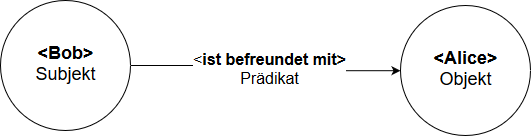
\includegraphics[width=0.75\textwidth]{img/triple.png}  
    \caption[ Semantic Web Stac]{ Semantic Web Stac}
  	\label{fig:triple}
\end{figure}
SCHREIBER und RAIMOND\footcite[Vgl.][]{schreiber2014rdf} erklären RDF in einem ausführlichen Beispiel an Hand folgenden Aussagen:
\\
\\
\textit{Bob ist eine Person.\\
Bob ist befreundet mit Alice.\\
Bob ist geboren am 4. Juli 1990. \\
Bob interessiert sich für die Mona Lisa.\\
Die Mona Lisa wurde von Leonardo da Vinci entworfen.}
\\
\\
Jede dieser Zeilen steht für ein Triple. \textit{Bob} ist Subjekt in vier der oben genannten Tripeln, \textit{Mona Lisa} tritt zweimal als Objekt und einmal als Subjekt auf. Dies ermöglicht es eine beliebige Menge an Triple zu einem komplexeren Graphen zusammenzusetzen und somit komplexere Sachverhalte beschreiben zu können. Abbildung \ref{fig:rdf_example} veranschaulicht das.
\begin{figure}[h]
  \centering
	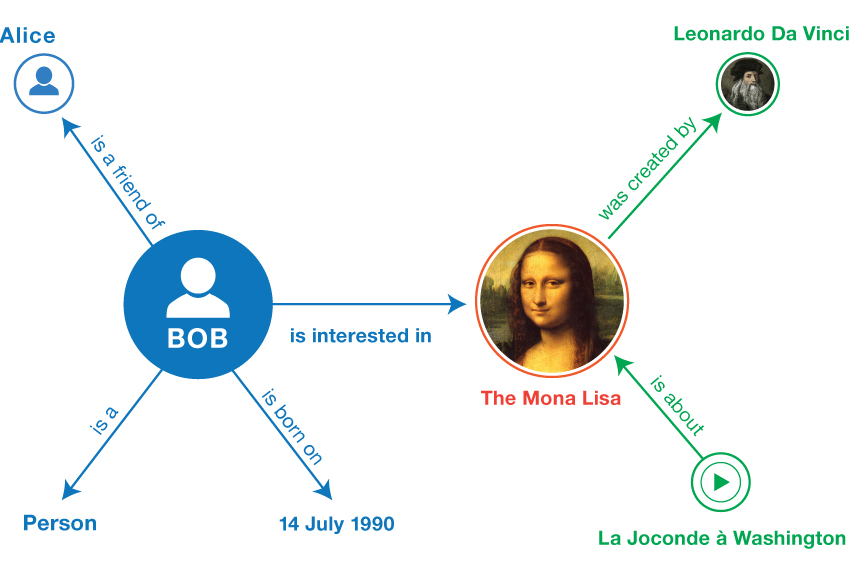
\includegraphics[width=1\textwidth]{img/rdf_example.png}  
    \caption[Visualisierung eines Graphen auf Basis eines RDF-Datensatz, \protect\url{https://www.w3.org/TR/rdf11-primer/}, 10.04.2019.]{Visualisierung eines Graphen auf Basis eines RDF-Datensatz.}
  	\label{fig:rdf_example}
\end{figure}
\textbf{\textit{Uniform Resource Identifier}(URI)} können in allen drei Positionen eines Triple erscheinen. Somit ist jeder Ressource, sowie jeder Beziehung zwischen Ressourcen durch eine URI identifizierbar. URI's sind durch ein erweiterbares Schema definiert, damit Ressourcen im Internet eindeutig adressiert werden können. Um dabei die Einheitlichkeit zu gewährleisten, folgen sie einem vordefinierten Satz von Syntaxregeln, der 5 Komponenten beinhaltet:\footcite[Vgl.][]{berners2004uniform}
\begin{center}
\textit{URI = scheme:[//authority]path[?query][\#fragment]}
\\
\end{center}
\begin{itemize}
\item \textbf{\textit{scheme}}: Definiert den Kontext und Typ. Bekannte Schemata sind beispielsweise die Webprotokolle \textit{Hyper Text Transfer Protocol} (http) oder das \textit{File Transfer Protocol} (ftp), sowie Notationskonzepte wie \textit{Uniform Resource Name} (URN)urn oder \textit{Digital Object Identifier} (doi).
\item \textbf{\textit{authority}}: Verwaltet Instanz in einem bestimmten vom Schema angegebenen Interpretationsraum, wie etwa das \textit{Domain Name System}.
\item \textbf{\textit{path}}: Der Pfad enthält – oft hierarchisch organisierte – Angaben, die zusammen mit dem Abfrageteil eine Ressource identifizieren. 
\item \textbf{\textit{query}}: Der Abfrageteil beinhaltet Daten zur Identifizierung von solchen Ressourcen, deren Ort durch die Pfadangabe allein nicht genau angegeben werden kann, wie beispielsweise ein Datensatz aus einer Datenbank, abgerufen werden
\item \textbf{\textit{fragment}}: Ist der optionale Fragmentbezeichner und referenziert eine Stelle innerhalb einer Ressource. Der Fragmentbezeichner bezieht sich immer nur auf den unmittelbar vorangehenden Teil des URI und wird von einem Hash (\#) eingeleitet.
\end{itemize}

Weiters werden URI in \textit{Uniform Resource Locator} (URL) und \textit{Uniform Resource Name} (URN) unterteilt. Wo URN Namen von Ressourcen eindeutig indetifuieren, wie etwa bei ISBN Nummern von Büchern, sind URL die gägnisten URI's, die den Ort einer Ressource addressieren und über einen Webbrowser auch aufrufen können.\footcite[Vgl.][S.21-22]{powers2003practical} Für das Triple \textit{<Bob>} \textit{<interessiert sich für>} \textit{<die Mona Lisa>} wird jeder Teilbestand eine URI und in der \textit{Turtle} Serialistion von RDF ergibt es folgenden Code:
\begin{lstlisting}[]
BASE   <http://example.org/>
PREFIX foaf: <http://xmlns.com/foaf/0.1/>
PREFIX xsd: <http://www.w3.org/2001/XMLSchema#>
PREFIX schema: <http://schema.org/>
PREFIX dcterms: <http://purl.org/dc/terms/>
PREFIX wd: <http://www.wikidata.org/entity/>

bob#me a foaf:Person ;
         foaf:knows <alice#me> ;
         schema:birthDate "1990-07-04"^^xsd:date ;
         foaf:topic_interest wd:Q12418 .
 
wd:Q12418 dcterms:title "Mona Lisa" ;
            dcterms:creator <http://dbpedia.org/resource/Leonardo_da_Vinci> .
\end{lstlisting}

%%%%%%%%%%%%%%%%%%%%%%%%%%%%%%%%%%%%%%%%%%%%%
%%%%%%%%%%%%%%%%%%%%%%%%%%%%%%%%%%%%%%%%%%%%%
\subsubsection{Resource Description Framework Schema (RDFs)}

Im vorhergehenden Beispiel wurden \textit{<Bob>} und \textit{<Alice>} der Klasse \textit{<Person>} zu geordnet. Sie sind Instanzen der Klasse \textit{<foaf:Person>}. Desweiteren wurde eine Relation zwischen diesen beiden Personen definiert: \textit{Bob ist befreundet mit Alice}.
\\
Um die Beziehungen zwischen Ressourcen zu beschreiben liefert das \textbf{Resource Description Framework Schema (RDFs)} eine semantische Erweiterung für RDF. Dies umfasst die Möglichkeit Klassen und Relationen, so genannte Properties, zu definieren und folgt dem Paradigma der Objektorientierung. Es lassen sich auf dieswe Weise Instanzen von Klassen erzeugen, die alle Eigenschaften der Klasse und ihrer übergeordneten Klassen erben. Blickt man auf das FOAF-Vokabular\footnote{FOAF-Specification, \protect\url{http://xmlns.com/foaf/spec/ }, 29.05.2019.}, das als RDFs umgesetzt ist, so kann man feststellen, dass \textit{foaf:Person} eine Unterklasse von \textit{foaf:Agent} ist. Weitere Unterklassen davon sind \textit{foaf:Group} und \textit{foaf:Organization}. Alle drei Unterklassen haben bestimmte Eigenschaft gemeinsam: sie setzen Handlungen in der Welt. Sie unterscheiden sich aber in den Relationen mit denen sie selbst, oder in Abgrenzung zu anderen Klassen, beschrieben werden können. Eine \textit{foaf:Group} besteht aus mehrern \textit{foaf:Person}. Dies wird mittels der Property \textit{foaf:member} ausgedrückt. Im Gegenzug verfügt \textit{foaf:Person} über eine Relation \textit{foaf:knows}, die ausdrückt, dass sich zwei Personen kennen. Die Richtung dieser Relation - wer wen kennt - wird mit den in RDFs mittels den Termen \textit{rdfs:Domain} und \textit{rdfs:Range} definiert. 
Für \textit{foaf:knows} wird \textit{Domain} und \textit{Range} auf die Klasse\textit{ foaf:Person} gesetzt: eine Person kennt eine andere Person. Für die Property \textit{foaf:member} wird \textit{Domain} auf \textit{foaf:Group} und \textit{Range} auf \textit{foaf:Person} gesetzt: eine Gruppe besteht aus Personen.
\\
Weiter führt RDFs Datentypen ein. Damit lässt sich beschreiben, um welche Art eines Literals es sich handelt. Es kann für die maschinelle Verarbeitung sehr wichtig sein zu wissen, ob es sich um eine Zeichenkette, eine Zahl, eine Datumsangabe oder eine XML Struktur handelt, da mit unterschiedlichen Datentypen andere Operationen einhergehen. 
\\
Mit den RDF Properties \textit{rdfs:label} und \textit{rdfs:comment} lassen sich Properties und Classes benennen und beschreiben. Das ist deswegen nötig, da der Fokus einer Klasse nur in bestimmten Kontexten Sinn macht. \textit{rdfs:label} definiert einen menschenlesbaren Namen einer Ressource. Es besteht stets die Möglichkeit in RDF die einzelnen Lables einer Ressource mit Sprachkürzel zu versehen. Die Property \textit{rdfs:comment} erlaubt es eine verbale Beschreibung zu einer Klasse hinzuzufügen.Am Beispiel von \textit{foaf:Person} ist das das Label ''Person'' und die Beschreibung:\\
'\textit{The Person class represents people. Something is a Person if it is a person. We don't nitpic about whether they're alive, dead, real, or imaginary. The Person class is a sub-class of the Agent class, since all people are considered 'agents' in FOAF. }''.\\
Daneben existiert auch ein Konstrukut \textit{rdfs:seeAlso}, um ausdrücken, dass es unter folgender URL noch weitere Information zu dieser Ressource gibt.\footcite{brickley2014rdf} Folgender Darstellung veranschaulicht die soeben beschriebenen Konstrukte in RDFs und zeigt Unterklassen der Superklasse \textit{foaf:Agent}, zwei Instanzen der Klasse \textit{foaf:Person} und stellt graphisch - durch den Pfeil - \textit{Domain} und \textit{Range} einer Propertie dar. 
\begin{figure}[H]
  \centering
	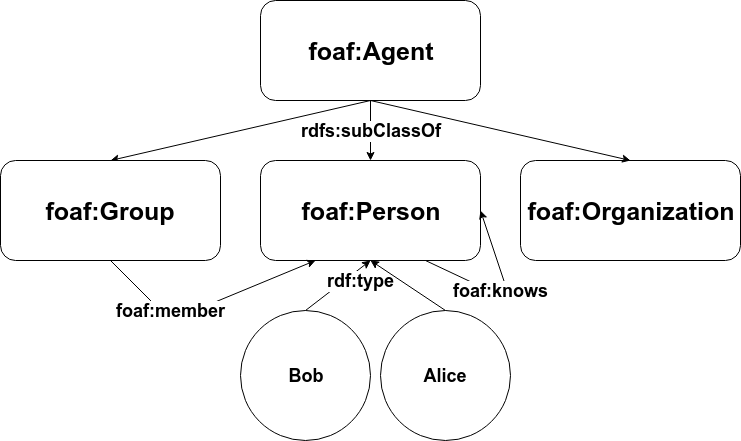
\includegraphics[width=0.75\textwidth]{img/rdfs.png}  
    \caption[RDFs-Beispiel auf Basis des FOAF-Vokabulars, eigene Darstellung.]{RDFs-Beispiel auf Basis des FOAF-Vokabulars}
  	\label{fig:web_stack}
\end{figure}
Hinter jeder Klasse, Property und  jeder Instanz steht eine URI. Folgendes RDF-Snippet zeigt wie die Klasse \textit{foaf:Person} und \textit{foaf:knows} im FOAF-Vokabular mittels RDFs definiert werden.
\begin{lstlisting}[]
@prefix rdfs: <http://www.w3.org/2000/01/rdf-schema#> .
PREFIX foaf: <http://xmlns.com/foaf/0.1/>
@prefix rdf: <http://www.w3.org/1999/02/22-rdf-syntax-ns#> .

foaf:Person a rdfs:Class ;
  rdfs:label "Person" ;
  rdfs:comment "A person." ;
  rdfs:subClassOf foaf:Agent .
  
foaf:knows a rdf:Property;
  rdfs:label "knows" ;
  rdfs:comment "A person known by this person (indicating some 
  level of reciprocated interaction between the parties)." ;
  rdfs:domain foaf:Person ;
  rdfs:range foaf:Person .
\end{lstlisting}

ToDo Hitzler\footcite[][]{hitzler2007semantic} 

%%%%%%%%%%%%%%%%%%%%%%%%%%%%%%%%%%%%%%%%%%%%%
%%%%%%%%%%%%%%%%%%%%%%%%%%%%%%%%%%%%%%%%%%%%%
\subsubsection{Taxonomien: Simple Knowledge Organisation (SKOS)}


%%%%%%%%%%%%%%%%%%%%%%%%%%%%%%%%%%%%%%%%%%%%%
%%%%%%%%%%%%%%%%%%%%%%%%%%%%%%%%%%%%%%%%%%%%%
\subsubsection{Abfragesprache: SPARQL}
Wie man in der Welt der relationalen Datenbanken mit der Abfragesprache SQL Datenbankabfragen formulieren kann, so kann man mit \textit{SPARQL Protocol And RDF Query Language} RDF Daten bzw. Triple in Graphdatenbanken abfragen.\footcite[][]{w3c2013sparql}
\\
Folgendes Snippet einer SPARQL-Abfrage zeigt die Syntax dieser Abfragesprache. Ziel dieser Abfrage ist es, alle Ressourcen in einer Graphdendatenbank abzufragen, die über eine \textit{foaf:name} und eine \textit{foaf:knows} Propertie verfügen. Das Ergebnis wird nach den Personen und Namen gruppiert, also es werden keine Dupletten von URI's zurückgegeben. Als Ausgabe erfolgt eine Tabelle (bzw. eine XML, JSON oder CSV Datenformat) in der die Namen und die Anzahl der Freunde, definiert als alle Knoten auf die \textit{foaf:know} referenziert.
\begin{lstlisting}[]
PREFIX foaf: <http://xmlns.com/foaf/0.1/>
SELECT ?name (COUNT(?friend) AS ?count)
WHERE { 
    ?person foaf:name ?name . 
    ?person foaf:knows ?friend . 
} GROUP BY ?person ?name
\end{lstlisting}
Mit PREFIX werden die Namespaces definiert. Das reservierte Wort \textit{SELECT} definiert alle Variabeln, diese werden durch ein vorangestelltes Fragezeichen gekennzeichnet, die als Rückgabewert definiert werden. Daneben gibt es in der SPARQL1.1 Version Operatoren und Funktionen, wie etwas \textit{COUNT()}, das alle Treffer der \textit{?friend} Variabel zählt und in der \textit{?count Variabel} speichert. Im \textit{WHERE} Bereich werden alle Bediengungen für die Abfrage definiert. Diese Bedienungen entsprechen der Definition eines Teilgraphen, der wiederum eine Teilmenge des gesamten Datenbestandes abbildet. Hier stehen weiter Konstrukte wie \textit{OPTIONAL}, einem logischen Oder, so wie \textit{UNION} einem logischen Und zur Verfügung. Über eine SPARQL-Endpoint können so User über das Web Datenbestände abfragen und mit diesen Arbeiten.\footcite[][S.1-45]{ducharme2013learning}  Ein bekanntes Beispiel dafür ist der Endpoint von Wikidata.

%%%%%%%%%%%%%%%%%%%%%%%%%%%%%%%%%%%%%%%%%%%%%
%%%%%%%%%%%%%%%%%%%%%%%%%%%%%%%%%%%%%%%%%%%%%
\subsection{Ontologien}
ToDO
\\
formationsmodelle umfassen die Verwendung einer expliziten Sprache zur Informationsdarstellung.\footcite{kobler2010qualitat} 
\\
\\
Der Gegenstandsbereich der \textbf{Ontologie als Disziplin in der Philosophie} umfasst alles, das existiert. Das Erkenntnisziel, so MEIXNER, ist auf allgemeiner begrifflicher Ebene zu finden und beschäftigt sich mit der Einteilung des Seins und den Grundstrukturen der Wirklichkeit, sowie der Frage nach dem Wesen der Existenz. Die Ontologie verfolgt nicht das Ziel Erkenntnis über ein Objekt zu erhalten, es beispielsweise zu vermessen oder zu beschreiben, sondern stellt sich die Frage nach welchen allgemeinen Kriterien Objekte im Verhältnis zu ontologischen Begriffen wie Sein, Aktualität, Universalie, Exemplifikation, Sachverhalt oder Individuum stehen.\footcite{meixner1994wissenschaft}
\\
Der Begriff \textbf{Ontologie in der Informationswissenschaft bzw. Informatik} umfasst ein pragmatisches Konzept zum Austausch und zur Wiederverwendung von formalisierten und gemeinschaftlich verwendeten Wissensstrukturen durch ein gemeinsames Vokabular. Ziel dabei ist es Informationssysteme zu implementieren. Die Spezifikation eines solchen Vokabulars für eine bestimmte Domäne nennt man Ontologie.
\\
Der Begriff wird in zwei Disziplinen mit jeweils unterschiedlichen Fokus verwendet. Dennoch sehe ich Gemeinsamkeiten. Beide setzen sich mit der Frage auseinander, wie  die Welt sinnvoll strukturiert werden kann, damit wir uns besser darin zurecht finden können. In diesem Kapitel wird die informationswissenschaftlichen Dimension des Ontologie-Begriffs und seiner Nutzung in den digitalen Geisteswissenschaften diskutiert und der Frage nachgehen, ob Ontologien ein geeignetes Werkzeug zur Formalisierung von geschichtswissenschaftlichen Domänen darstellen. Dabei soll anfangs "Wissen" kurz aus informationswissenschaftlicher Sicht definiert werden und über das semantische Netz eine Brücke zur Ontologie geschlagen werden. 

%%%%%%%%%%%%%%%%%%%%%%%%%%%%%%%%%%%%%%%%%%%%%
%%%%%%%%%%%%%%%%%%%%%%%%%%%%%%%%%%%%%%%%%%%%%
\subsubsection{Vom Wissen, über das Semantische Netz zur Ontologie}
\textbf{Wissen} ist eine systeminterne Repräsentation vorliegender Erfahrungen eines Menschen zu einem bestimmten Zeitpunkt, die einem zu überprüfenden Anspruch auf Gültigkeit ausgesetzt sein muss. Als solches prägt Wissen das Handeln und Denken eines Menschen auf den unterschiedlichsten Ebenen und dient zur Lösung von Problemen. Das jeweils aktuelle Wissen bildet einen kontextuellen Rahmen, in dem ankommende und bestehende Information interpretiert und zu neuen Erfahrungen verarbeitet werden.\footcite{favre2001information}
\\
Diese Definition von Wissen -- eine stärker informationswissenschaftliche -- hat seinen, neben vielen Definitionen in anderen Fachbereichen, legitimen Ursprung.  Unterschiedlichen Disziplinen haben andere Fragestellungen und benötigen dafür ein anderes theoretisches Gerüst. Ein Wissensbegriff in der Philosophie, beispielsweise, sollte viel weiter gefasst sein, als ein Wissensbegriff in der Informationswissenschaft, dessen Aufgabe darin besteht als Hilfsmittel in der Entwicklung und Umsetzung von Informationssystemen zu fungieren. 
\\
\\
Mittels Ontologie lässt sich ''Wissen'' als Netzwerk beschreiben. Ein Netzwerk ist ein gerichteter Graph, bestehend aus einer Menge von Knoten und einer Menge von Kanten, die die einzelnen Knoten miteinander verknüpfen. Damit lassen sich (fast) beliebige Entitäten und deren Verknüpfungen miteinander abbilden. Die Überlegungen zu einem \textbf{semantischen Netz}, als gedanklichen Vorgänger der Ontologie, stammen von QUILIIAN, der damit ein formales Erklärungsmodell für '\textit{die menschliche Repräsentation von Wissen über Worte und ihre Bedeutung als Netzwerk von Begriffen und ihren Relationen}' \footcite{stuckenschmidt2009ontologien} beschreibt. Semantische Netze können einen Kompromiss zwischen menschenverständlicher Repräsentation einer Domäne  und der formalen Verarbeitbarkeit durch eine Maschine darstellen.\footcite{reichenberger2010grundlagen} Das ist dadurch gegeben, dass die Struktur des Graphen (=Netz), sich einfach in Rechnern als Matrizen abbilden lässt.
\\
Die Ontologie ist eine Erweiterung des semantischen Netzes und nach GRUBER kann sie durch ein \textbf{4-Tupel} definiert werden. C ist eine Menge von \textbf{Klassen} (concepts, classes - Mengen von Entitäten aus der Realität), R eine Menge von \textbf{Relationen} (properties - Beziehungen zwischen Klassen), I eine Menge von \textbf{Instanzen} (individuals - einzelne Entität aus einer Menge) und A eine Menge von \textbf{Axiomen} (axioms - logische Regel).\footcite{joostbreukera2009flood} C und R lassen sich dabei stets als Graph abbilden. Ein Beispiel zur Veranschaulichung: 
\\
Es existiert eine Klasse (C) "Katzen", die mit der Relation "ist ein" (R) mit einer Klasse "Säugetier" verbunden ist.  Die Individuals (I) "Garfield“ und "Tom" sind Instanzen der Klasse "Katzen" und erben alle Eigenschaften, die in der Klasse "Katzen" definiert wurden. Eine Regel kann definiert werden (A), sodass immer wenn eine Klasse eine "ist ein" Verbindung zu einer Klasse wie "Säugetier" hat, es ausgeschlossen ist, dass es eine zweite "ist ein"-Verbindung  gibt, die auf eine andere Klasse wie etwa "Vögel" referenziert. 
\\
\\
Der Begriff der Ontologie terminologisch unscharfe verwendet.\footcite[Vgl.][S.1]{gruber1993translation} Die Unterschiede sind klein, aber dennoch entscheidend und sollen im Folgenden diskutiert werden.
Eine der  ersten  Definitionen des Begriffs der Ontologie stammt von GRUBER: 
\begin{center}
 "\textit{An ontology is    an    explicit    specification    of    a conceptualization}
"\footcite[][S.69]{hoekstra2009ontology}
\end{center}
Eine "\textit{conceptualization}" beschreibt den Prozess einer Vereinfachung, aber Fokussierung, eines bestimmten Aspekts der Realität. 
So kann eine Ontologie als Dokumentation eines 
wissen- schaftlichen 
Prozesses agieren, in dem die Wirklichkeit abstrahiert und reduziert wird und gleichzeitig die Domäne bzw. Forschungsfrage hervorgehoben und amplifiziert wird.\footcite[Vgl.][]{thaller2017ungefahre}
Unter "\textit{explicit}" versteht man, dass die Bedeutungen aller von der Ontologie erfassten Begriffe klar und eindeutig definiert sein müssen. Dies beinhaltet alle ihre Eigenschaften, Beschränkungen und Beziehungen, innerhalb, als auch außerhalb der Domäne.\footcite{sure2003methodology}
BORST erweitert GRUBERS Definition um  '\textit{formal  specification  of  a shared  conceptualization}'.\footcite{borst1997construction}
"\textit{Formal}" ergänzt dabei die Definition um die Notwendigkeit, dass Ontologien maschinenlesbar sein müssen. Erst diese Eigenschaft hebt sie von anderen Methoden zur Formalisierung von konzeptionellen Datenmodellen hervor. Der Zusatz "\textit{shared}" reflektiert die Tatsache, dass eine Ontologie Wissen erfasst, das durch den Konsens einer Gruppe - z.B. durch einen wissenschaftlichen  Diskurs - akzeptiert wird. Eine Ontologie darf nicht im Stillen von einer Person alleine entwickelt werden, sondern sollte in einem iterativen Prozess (Ontology Engineering) des Austausches und der Diskussion mit anderen entstehen. Ein solcher Prozess kann wie folgt ablaufen:
\begin{itemize}
\item Definition der Notwendigkeit und des Zieles einer Ontologie
\item Strukturierung des Wissens und konzeptionelle Entwicklung
\item Implementierung und Modellierung
\item Evaluierung und Dokumentation
\item Iteration dieser Punkte im Austausch mit anderen
\end{itemize}
Allgemeiner betrachtet definieren LINCKELS \& MEINEL eine Ontologie als ein Datenmodell zur Darstellung eines Sets miteinander vernetzter Konzepte innerhalb einer (Fach-)Domäne.\footcite{linckels2011librarian}
WELLER spricht von einer formalen und schematischen Darstellung einer Wissensdomäne auf Basis definierter Regeln und Vokabulars.\footcite{weller2013InformationBand}
\\ 
Zusammengefasst kann man sagen, dass sich mittels Ontologien komplexere Sachverhalte so darstellen lassen, dass Mensch und Maschinen in der Lage sind Strukturen, die durch eine Ontologie definierte und standardisierte sind, weiterverarbeiten zu können. Der Mehrwert kann vor allem in der Möglichkeit automatisierter Schlussfolgerungen, im Information Retrieval oder anderen formalen Methoden zur Verarbeitung von Daten liegen.
\\
\\
Der Ontology Editor Protégé erlaubt es, eine Ontologie und die darin enthaltenen Daten (Individuals) einem Reasoning - dem Abarbeiten aller Vorhanden Regeln in einer Ontologie auf Basis einer deskriptiven Logik - zu unterziehen. Für solche Zwecke gibt es natürlich auch API's und Bibliotheken in Programmiersprachen.\footcite{musen2015protege} Das Reasoning gilt als ein essentieller Baustein im Design, der Entwicklung, der Wartung und in der praktischen Anwendung einer Ontologie. Das Ergebnis davon sind Inferenzen. Inferenzen sind neu hergeleitete Schlussfolgerungen auf Basis der formalen Regeln einer Ontologie.\footcite{dentler2011comparison} Die Überprüfung strukturierter Daten mittels logischen Schlussfolgerungen kann dazu dienen, größere Datenmengen auf ihre Konsistenz und somit auch auf ihre Qualität hin zu prüfen, da logische Inkonsistenzen als Fehlermeldung angezeigt werden.
\\
\\
huhu Ontologie zitieren\footcite[Vgl][S.162-178]{jannidis2017digital} 


\section{Anwendung formaler Methoden auf Basis einer Ontologie}
\label{Umsetzung}

\subsection{Die Bookkeeping-Ontology als konzeptuelles Model für digitale Editionen von historischen Rechnungsbücher}
\label{BK}

MEDEA-Paper:
A CIDOC-CRM Based Ontology of Economic Activities
All these XML formats represent parts of what humans did when they exchanged goods and
services and recorded these economic activities in written form. Each method has its advantages.
But still it seems that behind all these forms is a common model which could be represented
conceptually in the following way: There are agents agreeing on a transfer of something
measurable and executing this transfer. Usually the transfer is mutual, i.e. at least two transfers
aggregate to a transaction, in which usually money is exchanged for commodities, services or
rights. Additionally one or the other party creates a documentation of this transfer, which can be
an artifact like a tally, but usually is a written accounting document. It is important to notice that
the financial document is not necessarily representing the transfer or the transaction itself; a
record can even be fictitious. It also adds a level of interpretation: The transactions are organized
in the document following a specific scheme meaningful to the agent commissioning the record,
the “categories”, “rubrics”, or “accounts”, which can be abstracted to dimensions; often the
accountant aggregates the individual transactions into totals, balancing the financial state or
demonstrating profits and losses; and some transactions are not recorded at all.
While the historical process of economic transactions can be modelled as seen above, the source
material thus has a complex relationship to these historical events we assume to have happened.
As in all manuscript analysis, a page is written by one or more hands (writers) in one or more
sessions. One specific record can be found on (parts of) one or more pages. So we have an
activity performed by one or more actors at a period of time, which may have been
discontinuous, which resulted in a record. The traces of this activity can be found in the
document and can be established as such by competent readers, as we have seen in the examples
above.
Each record represents a claim about something that happened in the real world, an economic
transaction of some sort. This is another activity, connected to but distinct from the record
creation event. In an event-based modelling of historical accounts these two activities will form
the core of a network of information, and information—about actors, time, location, the historical account document, and other events connected to the transaction such as goods,
money, currency information—become nodes attached to this core.
Formalizing the conceptual model resulting from these considerations would allow us to map the
formalizations described above for their procession as complete set. This goal seems reasonable
as of course the records of an economic activity in the ledger of one company should find their
counterpart in the ledger of its exchange partner. A meta search on digital representations of
various Hanse records could therefore allow extracting networks and flows of trade activities.
The research on long term price series or their regional diversion would profit from a common
access to the records. The recent solutions historians at the University of Tokyo (Kokaze et al,
2016) have found to represent chronology in historical accounts confirm this: They study the
relationship between agents mentioned in the accounts of the British Lay-Osborn Flotilla and
Chinese administration from the 1860s in time.
The conceptual model covers completely, what a TEI based transactionography (hsfr) and XBRL
encoding describe: The hfrs:transaction/medea:transaction consists of hfrs:transfers, each of
them involving medea:agents/@hfrs:fra and @hfrs:til. The hfrs:transfer is defined as ‘A transfer
of something of value’, which is a tei:measure/medea:measurable. The medea:documentation of
the transfer is encoded with hfrs:attested as a reference to a TEI text structure. The
hfrs:listAccount and hfrs:account express the interpretative organization of transactions in
medea:schemes and medea:dimensions. hfrs:listTransaction and hfrs:transferGrp are generic
grouping functionalities which are reflected in the medea:dimensions of documentation and the
medea:total and medea:balance concepts. The relationship between the suggested conceptual
model and the abstract level in XBRL is even more obvious: The XBRL 'financial facts' are a
superclass to medea:transfer, medea:transaction, or medea:total. They are recorded in 'instances'
(medea:document) and the 'taxonomies' describe their interpretative dimensions
(medea:dimension, medea:schema).
The currently most adaptable formal representation for this kind of data is the Resource
Description Framework (RDF) of the W3C. Its graph-based model is flexible but structured
enough to express complex data structures. The basic conceptualization similar to simple natural
language sentences as subject-predicate-object triples makes it fairly easy to understand. RDFs
and OWL7 offer rich possibilities for formal modelling. A preliminary RDFs schema for the
conceptual model has therefore been created and published on github
(\url{https://github.com/GVogeler/bookkeeping}).
The CIDOC-CRM, as an event-based ontology, is a good structure for encoding such
information, as shown through the use of the standard for several types of cultural-historical
evidence. As a matter of fact, it serves well to cover the main parts of the conceptual model
described above, with its two event types:
1. The creation of the accounting document
2. The transfer as the recorded economic activity
While the first is clearly a subclass of the E65\_Creation class, the latter can be considered as a
subtype of E7\_Activity and of E28\_Conceptual\_Object.
 Both are connected by the document
written by the accountant and attesting a transfer. The example from Kokaze et al. (2016)
demonstrates that the general properties of CIDOC-CRM events have practical research
relevance.
Given the specific need in modelling these documents and the activities documented in them,
some extensions to CIDOC-CRM should be made. This is also in line with what we have seen in
other areas including archaeological excavations8 and buildings,9 and scientific observations10
establishing a CIDOC-CRM based family of standards. In the development of this CIDOC-CRM
based extended model it will be an important question what the target for the modelling is, that
is, what time periods, geographical areas, and specific document types will function as evidence
for the modelling. This will determine how specific the model can be: the larger the scope, the
looser and more flexible the model must be.
The two event types described above have different relationships to truth. As for the records in
the historical account we know they exist and were written, at least as long as the original
document exists. What is questionable is who wrote it, when, and also the level of unity, that is,
what makes one record separate from other records. For the economic transaction documented in
the record the question of existence is somewhat different than from the record. We only know
there is a claim for an economic transaction, not that any transaction actually took place, for
which one often needs additional evidence, knowledge, and analysis to determine.
This creates an interesting question of modelling principles: should one model the worldview
expressed by the documents or should one express the worldview seen as most likely to be
correct by the historians (Ciula, Spence, Vieira 2008)? The choice of modelling standards should
not determine that choice. However, as CIDOC-CRM is a tool for information integration it is
more common to use it for models aiming towards historical truthfulness. That does not mean
that the worldview expressed in the documents should be hidden, just that the activities
expressed in the model will be the ones the historians believe to have taken place. Modelling and
encoding the transactions recorded in historical accounting documents as stand-off reference
between textual evidence and description of the economic and social ‘facts’ even makes possible
multiple interpretations of the textual evidence, which would lead to considering the addition of
a factoid-based approach (Bradley and Pasin 2015) to the model
Conclusions
The current results of the work done by the MEDEA collaborative are therefore fivefold:
1. The textual genre of accounts shows a great variety in form in its history with a
substantial common ground in concepts and human activities represented in these texts.
2. These concepts and human activities are of high interest in the humanities and historical
social science research.
3. Based on the work of the DH community in the TEI and of contemporary business
reporting standardization activities in XBRL, it is possible to develop a conceptual model
for the documentary representation of human activities in the field of economics.
4. This model can be expressed as a graph structure, and it can be integrated into the larger
conceptual framework of the CIDOC-CRM family of standards.
5. It is worthwhile to continue the development of the formal model and make suggestions
about how to integrate the formal model into encoding practice and data publication of
historical accounting records.
Certainly, the solutions discussed here are only a few of all the possible ways that web
technologies can enhance research with historical accounting records. The MEDEA scholars
look forward to suggestions for modifications of the ontology, additions of other possible
methods for encoding economic facts represented in accounting documents, more efficient setups
for execution of projects, and a thorough scrutiny of the conceptual consistency of our proposal.
The MEDEA scholars will continue their work on the ontology and will try to set up a collection
of examples showing how we think the integration of the representation of content expressed in
RDF and scholarly edition of accounting documents can be realized.\footcite[][S.9-12]{tomasekmedea}
\\
\\
Das abschließende Kapitel verbindet die theoretischen Überlegungen mit den technischen Ausführungen und skizziert die Arbeit, die im Zuge des Projektes \textbf{Digital Edition Publishing Cooperative for Historical Accounts (DEPCHA)}\footnote{\url{gams.uni-graz.at/depcha}} umgesetzt wurde. In diesem Projekt wird ein gemeinsamer Publikations-Hub für historische Rechnungsbücher implementiert. Im Zentrum steht die Entwicklung und Nutzung einer Ontologie, einer formalen Beschreibung eines konzeptuellen Models zur Standardisierung von Buchungstransaktionen in historischen Rechnungsunterlagen. Dabei wird ein im \textit{Web of Data}, sowie ein \textit{Linked Open Data} Zugang verfolgt. Das heißt, dass eben der Transkription und Edition der Rechnungsbücher, sowie der Verfügugnstellung der Digitalisate der Quellen, hochstrukturierte RDF-Daten existieren, die mittels der Bookkeeping-Ontologie formalisiert sind und Referenzen auf Normdaten und LOD-Vokabularien setzen. Mit diesem Zugang soll die Nachprüfbarkeit, die Sicherstellung und die Nachnutzbarkeit der Forschungsdaten und aller darauf aufbauenden quantitativen Methoden und deren Ergebnisse gewährleistet sein. Dabei spielt die Bookkeeping-Ontologie, im THALLER'schen Sinne als \textit{knowledge domain} eine zentrale Rolle. In diesem Kapitel soll zuerst auf die digitale Edition historischen Rechnungsbüchern und die dazu nötigen Standards, vor allem die TEI, eingegangen werden. Danach folgt die semantische Anreicherung und die Repräsentation der Inhalte in den Transaktionen, sowie eine detailierte Beschreibung der domänenspezifischen Bookkeeping-Ontology.  

\subsection{Digitale Edition von Historischen Rechnungsbüchern}
\subsubsection{Digitale Edition}
Eine Einführung

\subsubsection{Bookkeeping-Ontology}

Die \textit{Bookkeeping Ontology} ist ein konzeptionelles Modell zur formalen Beschreibung von Transaktionen in historischen Rechnungsunterlagen. Es wurde in einem Ontologie-Engineering-Prozess entwickelt, an dem Historiker*innen, Softwareentwickler*innen und digitale Geisteswissenschaftler*innen beteiligt waren.  \\
Eine Transaktion besteht aus mindestens einem Transfer. Jeder Transfer umfasst den Austausch von Dingen, die quantifizierbar sind, von einem Akteur zum anderen. Solche sogenannte \textit{Measurable} lassen sich in Geldbeträge, sowie wirtschaftliche Güter unterteilen. Geldbeträge sind dadurch gekennzeichnet, dass sie aus eine Zahl und einer Währung bestehen, wie etwa 10 US Dollar. Weiters gibt es spezielle Formen von Geldbeträgen, wie etwa Steuern, die eine einseitige Geldabgabe definieren, sowie Preise, die den monetären Wert eines Wirtschaftsgutes beschreiben. Die wirtschaftlichen Güter wiederum werden aufgeteilt in Waren -- bestehend aus Menge, Einheit und Art, wie 1 Sack Erdäpfel -- und Dienstleistungen, die eine zeitliche Komponente mit sich bringen können. Die Akteure diesen Transfers können Individuen, Gruppen, Organisationen oder Kontent sein. Die Ontologie erlaubt es explizit zu formulieren von wem an wen \textit{Measurable} transferiert werden.
\\
Weiters ist die Verbindung zur historischen Quelle bzw. zum jeweiligen Eintrag wichtiger Bestandteil der Ontologie. Ein Eintrag ist ein Informationsfragment und Beleg eines Ereignisses einer Transaktion in der Vergangenheit. Neben dieser Referenz besteht die Möglichkeit jede Transaktion in seiner zeitliche, räumliche und inhaltlichen Dimension, also der Zordnung zu einem bestimmten, durch die Forschungsfrage geprägten Kontext, zu beschreiben.
\\
Ein bk:Transfer kann von einem bk:Agent durchgeführt werden, also jemand übernimmt den Transferprozess. Bei der Verbuchung der Transaktion wird eine Transaktion im Sinne der doppelten Buchhaltung auf die Haben oder Soll Seite gebucht. 

\subsubsection{TEI Beispiele DEPCHA}


\begin{lstlisting}[]
@prefix bk: <https://gams.uni-graz.at/o:depcha.ontology> .

<#Transaction-0>
  a bk:Transaction> ;
  bk:consistsOf <#Transfer-1>, <#Transfer-2> ;
  bk:when "1808-08-01" ;
  bk:text "1/4 lb Powder 2/6 1 lb Shot 2/6 7 6" .

<#Transfer-1>
  a bk:Transfer ;
  bk:transfers <#Measurable-1> ;
  bk:from <#stagville> ;
  bk:to <#pers.2> .

<#Transfer-2>
  a bk:Transfer ;
  bk:transfers <#Measurable-2-1> ;
  bk:from <#pers.2> ;
  bk:to <#stagville> .

<#Measurable-1>
  a bk:Commodity ;
  bk:unit <wiki:Q100995> ;
  bk:quantity "0.25" ;
  bk:commodity <wikivQ2908004> ;
  bk:price <#Price-1> ;
  bk:text "1/4 lb Powder" .

<#Measurable-2-1>
  a bk:Money ;
  bk:unit <wiki:Q213142> ;
  bk:quantity "7" .
  
 <#pers.2>
  a bk:Between;
  bk:name "James Haley".
  
\end{lstlisting}

\begin{figure}[H]
\centering
	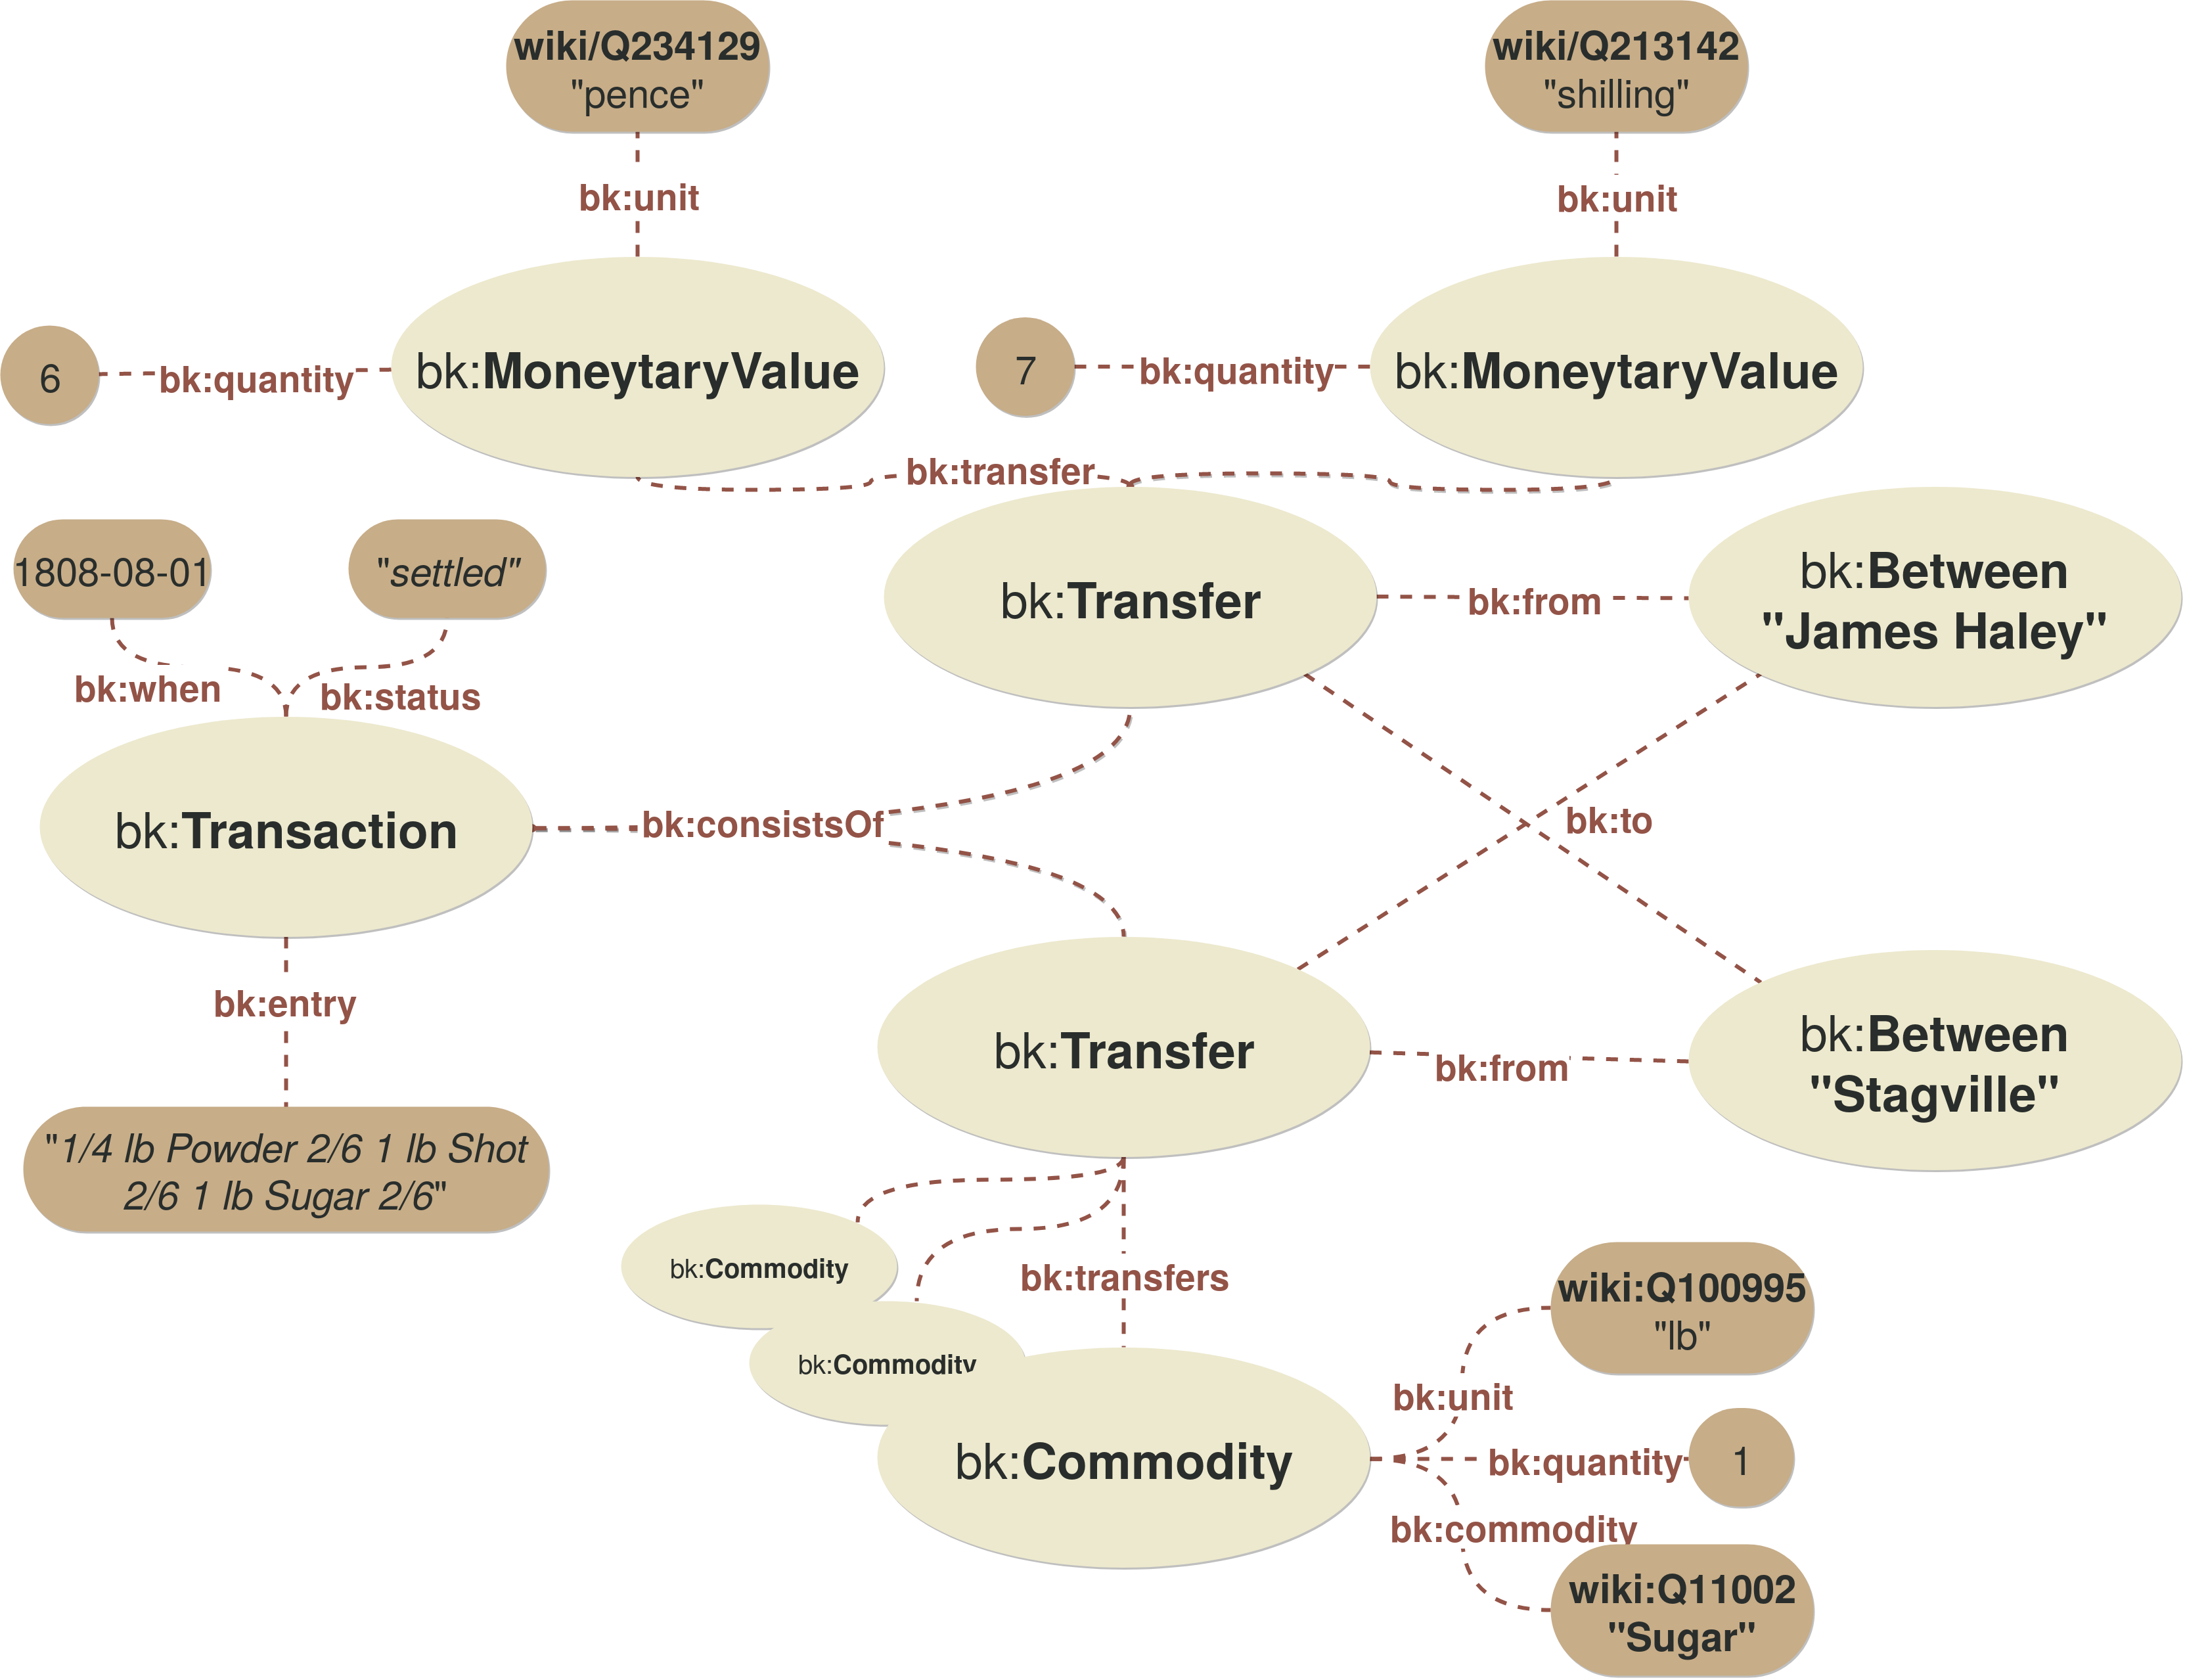
\includegraphics[width=0.75\textwidth]{img/example.png}  
    \caption[Graphische Darstellung des RDF, eigene Darstellung, 01.06.2019.]{Graphische Darstellung des RDF} \label{fig:example}
\end{figure}

\subsection{Informationsvisualisierung }

''\textit{The time of diagrammatic thinking is upon us. We need graphical interfaces for multidimensional and multimedia authoring that take advantage of computers’ abilities to aggregate, synthesize, and organize arguments along multiple axes}''\footcite[][S.119]{burdick2012digital_humanities}
\\
\\
Arbeitet man mit historischen Rechnungsbüchern, so arbeitet man mit einer Vielzahl von Informationsfragmenten. Für Forschungsfragen ist oft der Blick auf das Ganze interessant und so auf die Aggregation und Synthese der einzelnen Belge. BURDICK sieht gerde im Aufkommen der digitalen Geisteswissenschaften die Zeit reif die Ergebnisse der computgestützen Verarbeitung multidimensional zu Visualisieren. Die Informationsvisualisierung ist eine Methode, die dabei helfen kann Erklärungen historischer Ereignisse, die aus der Zusammenschau vieler Quellen und Entitäten zusammenkommen, zu argumentieren und sichtbar zu machen.\footcite[][S.3-5]{frank2018visualisierungswerkzeuge}
\\
\\
Als Visualisierung versteht man -- neben dem eigenständigen Fach aus dem Bereich \textit{Human-Computer Interaction} -- die Anwendung computerbasierter, interaktiver und visueller Repräsentation von abstrahierten Daten, die eine Hilfestellung bei der inhaltlichen Erfassung eines Themas liefern. Die Daten können sowohl quantitativer, geographische Koordinaten oder Messwerte, sowie qualitativer natur sein. Die Fachliteratur unterscheidet zwei Herangehensweisen. Wo die \textbf{Scientific Visualization} die Welt so darstellt, wie sie ist, beispielsweise die naturgetreue Darstellung des menschlichebn Körpers, wird in der \textbf{Information Visualization} ein Datenbestand in neuen (abstrakten) Räumen,  wie etwa in einem Koordinatensystem dargestellt. MUNZER fasst dies zusammen als "\textit{Its scientific visualization when the spatial representation is given. Its Information Visualization when the spatial represenation is chosen}''\footcite[][S.134-153)]{munzner2008process}. Im Falle von Rechnungsbüchern, und den Geschichtwissenschaften generell, kann man stets von einer Informationsvisualisierung ausgehen. Eine naturgetreue Darstellung historischer Ereignisse ist nie möglich.
\\
\\
FRANK führt 4 Beispiele von Projekten an, die die Methoden der Informationsvisualisierung so nutzen, dass sie zentraler Bestandteil zur Bearbeitung einer geisteswissenschaftlichen Forschungsfrage  und zur Überprüfung der Ergebnisse dient. Im politikwissenschaftlichen CEWS-Projekt (Alker et al., 2001) behandelt multiperspektivische Konfliktforschung und leistet seinen Beitrag zur Methoden- und Werkzeugentwicklung. So wird im Projekt Modallogik als formaler Rahmen für die kontrafaktische Analyse von möglichen Konfliktverläufen eingesetzt und die auf Husserl zurückgehende generative Phänomenologie wird zur Analyse der Perspektiven von historischen Akteuren (Konfliktparteien) auf Konfliktereignisse vorgeschlagen. Pellon (2010) kommt aus dem Bereich In
\\
\\
Gemeinsam haben alle diese Projekte, dass der Ausgangspunkt für die Visualisierung zum einen Daten sind, zum anderen ein Modell, dass den Daten Struktur verleiht und so die formale Verarbeitung in Hinblick auf eine Forschungsfrage erlaubt.
\\ 
\\
Sprache ist leichter als Bilder verwenden in einer Kommunikation.
\\
Wissensgewinnung durch Informations-Verbalisierung. 
\\
In der zwischenzeit brauchts neue Aggregatzustände für das Wissen. 
Datafication, die Dinge werden auch digital erfasst, neue Ansichten auf Daten und auf das Wissen.
\\
Wissensgewinnung durch Informationsvisualisierung
\\
Informationsvisualisierung dann, wenn man ein Thema nicht verbalisieren kann?
\\
Menschliche Wahrnehmung ist multimodal. Es entstehen unterschiedliche Repräsentation in unserem Bewusstsein von aufgenommenen Wahrnehmungen. Ein produktives Wechselverhältnis herstellen zwischen Sprache und Text.
\\
Close Viewing: Blick auf einen Eintrag
Distant Viewing: Blick auf alle EInträge
\\
Können wir da was draus lernen? Aus der distan viewing darstellung?
\\
Übersetzung eines Themas in Daten und die Übersetzung der Daten in Bilder.
Wie soll das Interface aussehen am Ende: in Beschreibungen, Skizzen und Worten.
\\
Ein Blick ist selten genug: Multiple Views
Das Prinzip der Multiperspektivität.
\\
Information-Seeking-Mantra: Ben Shneiderman (in frühesten Tagen sich bereits damit beschäftigt)
\\
Overview first            ein Orientierungswissen anbieten
 then zoom and filter        das interssiert mich vl
Details on demand        damit arbeite ich
\\
Informationsvisualisierung will nicht (nur) hübsch sein, sondern Problemstellungen lösen.
\\
Visuelle Repräsentationen können einerseits auf ein realistische Bild hinziehen (Dinge nachmodellieren), oder diagrammtisch (in einer andere Sprache überführen, mit einer Syntax und einer Semantik; menschengemacht)
\\ 
Scientific Visualization und Information Visualization
\\
A Tour through the Visualization Zoo (Jeffrey Heer, Michael Bostock et. al. 2010)
\\
Visualization are also interesting for non-expert users.
Because while they are interacting with them, their pattern-mind is learning. Even thoug they dont know the numbers behind that. [Valdis Krebs, 2011]
\\
Papers:
\\
Choreographien der Existenz: Zur multimodalen Erweiterung biographischer Forschung und Lehre durch Verfahren der visuellen Analyse und Synthese
\\
Visualization of Cultural Heritage Collection Data: State of the Art and Future Challenges
\\
Paper:
Distributed Cognition as a Theoretical Framework for Information Visualization
\\
\\
“The purpose of information visualization is to amplify cognitive performance, not just to create interesting pictures.”
\\
“Information visualization should do for the mind what automobiles do for the feed.
[Card et. al 2008, p.539]
\\
Es ist die Rede von einer Synergie zwischen Kognition und Computer.
\\
Wo sind die Grenzen und Herausforderungen der menschlichen Aufnahmefähigkeit.
Things far away, in the past, in the future, very large - very small.
\\
Komplexität: viele Elemente, unterschiedlicher Art haben viele Relationen 
multidimensional , multivariable und kann auch noch dynamisch sein.
Überall brauchen wir Visualisierung nicht, sondern nur da, wo die Komplexität größer ist.  
Definition des Begriffes der Komplexität, aus der Komplexitätsforschungs.
\\
Historische Rechnungsbücher = das Ganze
Elemente: 
Transaktionen
Transfer
Akteure
Güter, Dienstleistungen, als Wirtschaftsgüter
Geldbeträge Preise und Steuern 
Datum
\\
Beziehungen:
Von nach
Wieviel, Währung, Maßeinheit
\\
Für die Informationsvisualisierung ist es wichtig zuerst ein konzeptuelles Modell zu entwickeln und durchdenken, um daraus die Anwendungsszenarien ableiten zu können.
\\
SciVis - InfoVis
\\
\\
Wenn die räumliche Einordnung gegeben ist, wenn die räumliche Darstellung erst geschaffen wird. 
\\
Auch ein Fotoapparat macht SciVis
\\
Worlds, not stories, paper [Moritz Stefaner]
\\
Informationsvisualisierung ist die Welt nur mit anderen Regeln repräsentiert, um abstrakte Daten sichtbar zu machen.
\\
Microsoft timelinestoryteller
\\
Alle Einträge-Datum + Legende = alle Personen.
\\
\\
Treemap
\\
Inspiriert durch tree diagram: also folder mit underfolder;
\\
Es gibt Mengen. Die sind Rechtecke, und je größer dei Menge, desto größer die Rechtecke. Und alle darin befindlichen Untermengen (Säugetierte -> Hund, -> Katze) sind im Rechteck und zeigen, wie viel Platz sie innerhalb der übermenge einnehmen.
\\
Hierachien, Vergleichn, Teil eines Ganzen
\\
Rechnungsbuch: Alle Einträge und die WirtschaftsGüter in einer Hierachie: 
\\
Alle Lebensmittel, darin sind die Erdäpgel, mais
Alle Textillen Produkte: Kleidung
Alle Dienstleistungen - Arbeit, 
\\
Graphs, Maps, Trees: Franco Moretti 





\subsubsection{Statistische Auswertung}

\section{Textfragmente}

Das \textit{Data for History Consortium}\footcite{beretta2017dataforhistory} geht einen vergleichbaren Weg und versucht ein gemeinsames Set an Methoden im \textit{Web of Data} zu entwickeln, um Daten in den Geschichtswissenschaften zu modellieren, verknüpfen und auszutauschen.
\\
\\
hehe\footcite[Vgl.][]{sahle2013digitale}
huhu\footcite[Vgl][S.234-252]{jannidis2017digital} 
\\
Kapitel in dem digitale Edition, TEI und How to Bookkeep behandelt wird. Und die besonderheiten editorische Arbeit mit Rechnungsbüchern. 
\\
TOMASEK und BAUMAN beschreiben ein Modell eines interpretativen Markups, um Beziehungen zwischen Individueen, Geld- Güter- und Dienstleistungstransfer, die Doppeleintrag-Buchhaltung umfassenm auszuzeichnen. Die Auszeichnung basiert auf den ausdrucksstarken Richtlinien der TEI. \footcite[Vgl.][S.1-2, \protect\url{http://journals.openedition.org/jtei/895}, 08.03.2018]{tomasek2013encoding}
\footcite[][S.41-44]{kobler2010qualitat}


\section{Zusammenfassung}

\newpage
\bibliographystyle{jurabib}
\bibliography{literatur}
\newpage
\listoffigures

\end{document}
